\documentclass[twoside]{article}

% Packages required by doxygen
\usepackage{calc}
\usepackage{doxygen}
\usepackage{graphicx}
\usepackage[utf8]{inputenc}
\usepackage{makeidx}
\usepackage{multicol}
\usepackage{multirow}
\usepackage{textcomp}
\usepackage[table]{xcolor}

% NLS support packages
\usepackage[ngerman]{babel}

% Font selection
\usepackage[T1]{fontenc}
\usepackage{mathptmx}
\usepackage[scaled=.90]{helvet}
\usepackage{courier}
\usepackage{amssymb}
\usepackage{sectsty}
\renewcommand{\familydefault}{\sfdefault}
\allsectionsfont{%
  \fontseries{bc}\selectfont%
  \color{darkgray}%
}
\renewcommand{\DoxyLabelFont}{%
  \fontseries{bc}\selectfont%
  \color{darkgray}%
}

% Page & text layout
\usepackage{geometry}
\geometry{%
  a4paper,%
  top=2.5cm,%
  bottom=2.5cm,%
  left=2.5cm,%
  right=2.5cm%
}
\tolerance=750
\hfuzz=15pt
\hbadness=750
\setlength{\emergencystretch}{15pt}
\setlength{\parindent}{0cm}
\setlength{\parskip}{0.2cm}
\makeatletter
\renewcommand{\paragraph}{%
  \@startsection{paragraph}{4}{0ex}{-1.0ex}{1.0ex}{%
    \normalfont\normalsize\bfseries\SS@parafont%
  }%
}
\renewcommand{\subparagraph}{%
  \@startsection{subparagraph}{5}{0ex}{-1.0ex}{1.0ex}{%
    \normalfont\normalsize\bfseries\SS@subparafont%
  }%
}
\makeatother

% Headers & footers
\usepackage{fancyhdr}
\pagestyle{fancyplain}
\fancyhead[LE]{\fancyplain{}{\bfseries\thepage}}
\fancyhead[CE]{\fancyplain{}{}}
\fancyhead[RE]{\fancyplain{}{\bfseries\leftmark}}
\fancyhead[LO]{\fancyplain{}{\bfseries\rightmark}}
\fancyhead[CO]{\fancyplain{}{}}
\fancyhead[RO]{\fancyplain{}{\bfseries\thepage}}
\fancyfoot[LE]{\fancyplain{}{}}
\fancyfoot[CE]{\fancyplain{}{}}
\fancyfoot[RE]{\fancyplain{}{\bfseries\scriptsize Erzeugt am Die Nov 5 2013 23\-:44\-:56 für $<$sep13$>$ von Doxygen }}
\fancyfoot[LO]{\fancyplain{}{\bfseries\scriptsize Erzeugt am Die Nov 5 2013 23\-:44\-:56 für $<$sep13$>$ von Doxygen }}
\fancyfoot[CO]{\fancyplain{}{}}
\fancyfoot[RO]{\fancyplain{}{}}
\renewcommand{\footrulewidth}{0.4pt}
\renewcommand{\sectionmark}[1]{%
  \markright{\thesection\ #1}%
}

% Indices & bibliography
\usepackage{natbib}
\usepackage[titles]{tocloft}
\setcounter{tocdepth}{3}
\setcounter{secnumdepth}{5}
\makeindex

% Hyperlinks (required, but should be loaded last)
\usepackage{ifpdf}
\ifpdf
  \usepackage[pdftex,pagebackref=true]{hyperref}
\else
  \usepackage[ps2pdf,pagebackref=true]{hyperref}
\fi
\hypersetup{%
  colorlinks=true,%
  linkcolor=blue,%
  citecolor=blue,%
  unicode%
}

% Custom commands
\newcommand{\clearemptydoublepage}{%
  \newpage{\pagestyle{empty}\cleardoublepage}%
}


%===== C O N T E N T S =====

\begin{document}

% Titlepage & ToC
\hypersetup{pageanchor=false}
\pagenumbering{roman}
\begin{titlepage}
\vspace*{7cm}
\begin{center}%
{\Large $<$sep13$>$ }\\
\vspace*{1cm}
{\large Erzeugt von Doxygen 1.8.5}\\
\vspace*{0.5cm}
{\small Die Nov 5 2013 23:44:56}\\
\end{center}
\end{titlepage}
\tableofcontents
\pagenumbering{arabic}
\hypersetup{pageanchor=true}

%--- Begin generated contents ---
\section{Hierarchie-\/\-Verzeichnis}
\subsection{Klassenhierarchie}
Die Liste der Ableitungen ist -\/mit Einschränkungen-\/ alphabetisch sortiert\-:\begin{DoxyCompactList}
\item \contentsline{section}{Ruleset.\-Card}{\pageref{a00002}}{}
\begin{DoxyCompactList}
\item \contentsline{section}{Ruleset.\-Hearts\-Card}{\pageref{a00047}}{}
\item \contentsline{section}{Ruleset.\-Wizard\-Card}{\pageref{a00085}}{}
\end{DoxyCompactList}
\item \contentsline{section}{Ruleset.\-Card\-Deck}{\pageref{a00003}}{}
\item \contentsline{section}{Ruleset.\-Card\-Deck\-Builder}{\pageref{a00004}}{}
\item \contentsline{section}{Client.\-Card\-I\-D}{\pageref{a00005}}{}
\item \contentsline{section}{Client.\-Client\-Controller}{\pageref{a00008}}{}
\item \contentsline{section}{Client.\-Client\-Main}{\pageref{a00012}}{}
\item \contentsline{section}{Ruleset.\-Client\-Ruleset}{\pageref{a00014}}{}
\begin{DoxyCompactList}
\item \contentsline{section}{Ruleset.\-Client\-Hearts}{\pageref{a00009}}{}
\item \contentsline{section}{Ruleset.\-Client\-Wizard}{\pageref{a00016}}{}
\end{DoxyCompactList}
\item \contentsline{section}{Client.\-Client\-State}{\pageref{a00015}}{}
\item \contentsline{section}{Ruleset.\-Colour}{\pageref{a00017}}{}
\item \contentsline{section}{Com\-Objects.\-Com\-Been\-Kicked}{\pageref{a00018}}{}
\item \contentsline{section}{Client.\-View.\-Discard\-Pile}{\pageref{a00036}}{}
\item \contentsline{section}{Client.\-View.\-Draw\-Deck}{\pageref{a00037}}{}
\item \contentsline{section}{Ruleset.\-Game\-Client\-Update}{\pageref{a00039}}{}
\item \contentsline{section}{Ruleset.\-Game\-Phase}{\pageref{a00042}}{}
\item \contentsline{section}{Server.\-Game\-Server\-Representation}{\pageref{a00044}}{}
\item \contentsline{section}{Ruleset.\-Game\-State}{\pageref{a00045}}{}
\item \contentsline{section}{Ruleset.\-Hearths\-Deck}{\pageref{a00046}}{}
\item \contentsline{section}{Ruleset.\-Hearts\-I\-D}{\pageref{a00050}}{}
\item \contentsline{section}{Client.\-View.\-Language}{\pageref{a00052}}{}
\item \contentsline{section}{Client.\-Message\-Listener\-Thread}{\pageref{a00056}}{}
\item \contentsline{section}{Com\-Objects.\-Msg\-Card\-Request}{\pageref{a00058}}{}
\item \contentsline{section}{Client.\-M\-V\-Messages}{\pageref{a00068}}{}
\item \contentsline{section}{Ruleset.\-Other\-Data}{\pageref{a00069}}{}
\begin{DoxyCompactList}
\item \contentsline{section}{Ruleset.\-Hearts\-Data}{\pageref{a00049}}{}
\item \contentsline{section}{Ruleset.\-Wiz\-Data}{\pageref{a00088}}{}
\end{DoxyCompactList}
\item \contentsline{section}{Client.\-View.\-Other\-Player}{\pageref{a00070}}{}
\item \contentsline{section}{Client.\-View.\-Own\-Hand}{\pageref{a00071}}{}
\item \contentsline{section}{Ruleset.\-Player\-State}{\pageref{a00074}}{}
\item \contentsline{section}{Ruleset.\-Ruleset\-Type}{\pageref{a00076}}{}
\item Runnable\begin{DoxyCompactList}
\item \contentsline{section}{Server.\-Client\-Listener\-Thread}{\pageref{a00010}}{}
\item \contentsline{section}{Server.\-Lobby\-Server.\-Client\-Listener\-Thread}{\pageref{a00011}}{}
\item \contentsline{section}{Server.\-Player}{\pageref{a00073}}{}
\end{DoxyCompactList}
\item \contentsline{section}{Server.\-Server}{\pageref{a00078}}{}
\begin{DoxyCompactList}
\item \contentsline{section}{Server.\-Game\-Server}{\pageref{a00043}}{}
\item \contentsline{section}{Server.\-Lobby\-Server}{\pageref{a00054}}{}
\end{DoxyCompactList}
\item \contentsline{section}{Server.\-Server\-Main}{\pageref{a00080}}{}
\item \contentsline{section}{Ruleset.\-Server\-Ruleset}{\pageref{a00081}}{}
\begin{DoxyCompactList}
\item \contentsline{section}{Ruleset.\-Server\-Hearts}{\pageref{a00079}}{}
\item \contentsline{section}{Ruleset.\-Server\-Wizard}{\pageref{a00082}}{}
\end{DoxyCompactList}
\item \contentsline{section}{Client.\-View\-Notification}{\pageref{a00083}}{}
\item \contentsline{section}{Ruleset.\-Wizard\-Deck}{\pageref{a00086}}{}
\item \contentsline{section}{Ruleset.\-Wiz\-I\-D}{\pageref{a00089}}{}
\item J\-Frame\begin{DoxyCompactList}
\item \contentsline{section}{Client.\-View.\-Create\-Game}{\pageref{a00035}}{}
\item \contentsline{section}{Client.\-View.\-Game}{\pageref{a00038}}{}
\item \contentsline{section}{Client.\-View.\-Game\-Lobby}{\pageref{a00040}}{}
\item \contentsline{section}{Client.\-View.\-Lobby}{\pageref{a00053}}{}
\item \contentsline{section}{Client.\-View.\-Login}{\pageref{a00055}}{}
\item \contentsline{section}{Client.\-View.\-Password}{\pageref{a00072}}{}
\end{DoxyCompactList}
\item J\-Label\begin{DoxyCompactList}
\item \contentsline{section}{Client.\-View.\-Card}{\pageref{a00001}}{}
\begin{DoxyCompactList}
\item \contentsline{section}{Client.\-View.\-Hearts\-Card}{\pageref{a00048}}{}
\item \contentsline{section}{Client.\-View.\-Wiz\-Card}{\pageref{a00087}}{}
\end{DoxyCompactList}
\end{DoxyCompactList}
\item J\-Panel\begin{DoxyCompactList}
\item \contentsline{section}{Client.\-View.\-Game\-Panel}{\pageref{a00041}}{}
\end{DoxyCompactList}
\item Observable\begin{DoxyCompactList}
\item \contentsline{section}{Client.\-Client\-Model}{\pageref{a00013}}{}
\end{DoxyCompactList}
\item Observer\begin{DoxyCompactList}
\item \contentsline{section}{Client.\-View.\-Choose\-Cards}{\pageref{a00006}}{}
\item \contentsline{section}{Client.\-View.\-Choose\-Item}{\pageref{a00007}}{}
\item \contentsline{section}{Client.\-View.\-Create\-Game}{\pageref{a00035}}{}
\item \contentsline{section}{Client.\-View.\-Game}{\pageref{a00038}}{}
\item \contentsline{section}{Client.\-View.\-Game\-Lobby}{\pageref{a00040}}{}
\item \contentsline{section}{Client.\-View.\-Input\-Number}{\pageref{a00051}}{}
\item \contentsline{section}{Client.\-View.\-Lobby}{\pageref{a00053}}{}
\item \contentsline{section}{Client.\-View.\-Login}{\pageref{a00055}}{}
\item \contentsline{section}{Client.\-View.\-Password}{\pageref{a00072}}{}
\item \contentsline{section}{Client.\-View.\-Score\-Window}{\pageref{a00077}}{}
\item \contentsline{section}{Client.\-View.\-Warning}{\pageref{a00084}}{}
\end{DoxyCompactList}
\item Serializable\begin{DoxyCompactList}
\item \contentsline{section}{Com\-Objects.\-Com\-Object}{\pageref{a00029}}{}
\begin{DoxyCompactList}
\item \contentsline{section}{Com\-Objects.\-Com\-Chat\-Message}{\pageref{a00019}}{}
\item \contentsline{section}{Com\-Objects.\-Com\-Client\-Leave}{\pageref{a00020}}{}
\item \contentsline{section}{Com\-Objects.\-Com\-Client\-Quit}{\pageref{a00021}}{}
\item \contentsline{section}{Com\-Objects.\-Com\-Create\-Game\-Request}{\pageref{a00022}}{}
\item \contentsline{section}{Com\-Objects.\-Com\-Init\-Game\-Lobby}{\pageref{a00023}}{}
\item \contentsline{section}{Com\-Objects.\-Com\-Init\-Lobby}{\pageref{a00024}}{}
\item \contentsline{section}{Com\-Objects.\-Com\-Join\-Request}{\pageref{a00025}}{}
\item \contentsline{section}{Com\-Objects.\-Com\-Kick\-Player\-Request}{\pageref{a00026}}{}
\item \contentsline{section}{Com\-Objects.\-Com\-Lobby\-Update\-Gamelist}{\pageref{a00027}}{}
\item \contentsline{section}{Com\-Objects.\-Com\-Login\-Request}{\pageref{a00028}}{}
\item \contentsline{section}{Com\-Objects.\-Com\-Ruleset}{\pageref{a00030}}{}
\item \contentsline{section}{Com\-Objects.\-Com\-Server\-Acknowledgement}{\pageref{a00031}}{}
\item \contentsline{section}{Com\-Objects.\-Com\-Start\-Game}{\pageref{a00032}}{}
\item \contentsline{section}{Com\-Objects.\-Com\-Update\-Playerlist}{\pageref{a00033}}{}
\item \contentsline{section}{Com\-Objects.\-Com\-Warning}{\pageref{a00034}}{}
\end{DoxyCompactList}
\item \contentsline{section}{Com\-Objects.\-Ruleset\-Message}{\pageref{a00075}}{}
\begin{DoxyCompactList}
\item \contentsline{section}{Com\-Objects.\-Msg\-Card}{\pageref{a00057}}{}
\item \contentsline{section}{Com\-Objects.\-Msg\-Game\-End}{\pageref{a00059}}{}
\item \contentsline{section}{Com\-Objects.\-Msg\-Multi\-Cards}{\pageref{a00060}}{}
\item \contentsline{section}{Com\-Objects.\-Msg\-Multi\-Cards\-Request}{\pageref{a00061}}{}
\item \contentsline{section}{Com\-Objects.\-Msg\-Multiple\-Cards\-Request}{\pageref{a00062}}{}
\item \contentsline{section}{Com\-Objects.\-Msg\-Number}{\pageref{a00063}}{}
\item \contentsline{section}{Com\-Objects.\-Msg\-Number\-Request}{\pageref{a00064}}{}
\item \contentsline{section}{Com\-Objects.\-Msg\-Selection}{\pageref{a00065}}{}
\item \contentsline{section}{Com\-Objects.\-Msg\-Selection\-Request}{\pageref{a00066}}{}
\item \contentsline{section}{Com\-Objects.\-Msg\-User}{\pageref{a00067}}{}
\end{DoxyCompactList}
\end{DoxyCompactList}
\end{DoxyCompactList}

\section{Klassen-\/\-Verzeichnis}
\subsection{Auflistung der Klassen}
Hier folgt die Aufzählung aller Klassen, Strukturen, Varianten und Schnittstellen mit einer Kurzbeschreibung\-:\begin{DoxyCompactList}
\item\contentsline{section}{\hyperlink{a00001}{Client.\-View.\-Card} \\*\hyperlink{a00001}{Card} ist die View-\/seitige Repräsentation einer Karte }{\pageref{a00001}}{}
\item\contentsline{section}{\hyperlink{a00002}{Ruleset.\-Card} \\*Diese Klasse modelliert eine Spielkarte }{\pageref{a00002}}{}
\item\contentsline{section}{\hyperlink{a00003}{Ruleset.\-Card\-Deck} }{\pageref{a00003}}{}
\item\contentsline{section}{\hyperlink{a00004}{Ruleset.\-Card\-Deck\-Builder} }{\pageref{a00004}}{}
\item\contentsline{section}{\hyperlink{a00005}{Client.\-Card\-I\-D} }{\pageref{a00005}}{}
\item\contentsline{section}{\hyperlink{a00006}{Client.\-View.\-Choose\-Cards} }{\pageref{a00006}}{}
\item\contentsline{section}{\hyperlink{a00007}{Client.\-View.\-Choose\-Item} \\*Dieses Fenster ermöglicht es dem Spieler aus einer Liste von Items eines auszuwählen }{\pageref{a00007}}{}
\item\contentsline{section}{\hyperlink{a00008}{Client.\-Client\-Controller} }{\pageref{a00008}}{}
\item\contentsline{section}{\hyperlink{a00009}{Ruleset.\-Client\-Hearts} \\*Diese Klasse bildet das Regelwerk für den Client bei einer Partie Hearts }{\pageref{a00009}}{}
\item\contentsline{section}{\hyperlink{a00010}{Server.\-Client\-Listener\-Thread} }{\pageref{a00010}}{}
\item\contentsline{section}{\hyperlink{a00011}{Server.\-Lobby\-Server.\-Client\-Listener\-Thread} \\*Diese Klasse ist für das Zustandekommen von Clientverbindungen zuständig }{\pageref{a00011}}{}
\item\contentsline{section}{\hyperlink{a00012}{Client.\-Client\-Main} \\*Die \hyperlink{a00012}{Client\-Main} Klasse startet den Spielclient und initialisiert dessen Komponenten }{\pageref{a00012}}{}
\item\contentsline{section}{\hyperlink{a00013}{Client.\-Client\-Model} \\*Implementiert das Client Model }{\pageref{a00013}}{}
\item\contentsline{section}{\hyperlink{a00014}{Ruleset.\-Client\-Ruleset} \\*\hyperlink{a00014}{Client\-Ruleset} ist eine abstrakte Klasse und wird zur Regelvorauswertung im Client verwendet }{\pageref{a00014}}{}
\item\contentsline{section}{\hyperlink{a00015}{Client.\-Client\-State} \\*Dieser Enumerator enthält alle Zustände in denen sich der Client befinden kann }{\pageref{a00015}}{}
\item\contentsline{section}{\hyperlink{a00016}{Ruleset.\-Client\-Wizard} \\*Diese Klasse bildet das Regelwerk für den Client bei einer Partie Wizard }{\pageref{a00016}}{}
\item\contentsline{section}{\hyperlink{a00017}{Ruleset.\-Colour} \\*Repräsentiert die Farbe einer Karte }{\pageref{a00017}}{}
\item\contentsline{section}{\hyperlink{a00018}{Com\-Objects.\-Com\-Been\-Kicked} \\*Diese Klasse ist ein spezielles Kommunikations-\/\-Objekt }{\pageref{a00018}}{}
\item\contentsline{section}{\hyperlink{a00019}{Com\-Objects.\-Com\-Chat\-Message} \\*Diese Klasse ist ein spezielles Kommunikations-\/\-Objekt }{\pageref{a00019}}{}
\item\contentsline{section}{\hyperlink{a00020}{Com\-Objects.\-Com\-Client\-Leave} \\*Diese Klasse ist ein spezielles Kommunikations-\/\-Objekt }{\pageref{a00020}}{}
\item\contentsline{section}{\hyperlink{a00021}{Com\-Objects.\-Com\-Client\-Quit} \\*Diese Klasse ist ein spezielles Kommunikations-\/\-Objekt }{\pageref{a00021}}{}
\item\contentsline{section}{\hyperlink{a00022}{Com\-Objects.\-Com\-Create\-Game\-Request} \\*Diese Klasse ist ein spezielles Kommunikations-\/\-Objekt }{\pageref{a00022}}{}
\item\contentsline{section}{\hyperlink{a00023}{Com\-Objects.\-Com\-Init\-Game\-Lobby} \\*Diese Klasse ist ein spezielles Kommunikations-\/\-Objekt }{\pageref{a00023}}{}
\item\contentsline{section}{\hyperlink{a00024}{Com\-Objects.\-Com\-Init\-Lobby} \\*Diese Klasse ist ein spezielles Kommunikations-\/\-Objekt }{\pageref{a00024}}{}
\item\contentsline{section}{\hyperlink{a00025}{Com\-Objects.\-Com\-Join\-Request} \\*Diese Klasse ist ein spezielles Kommunikations-\/\-Objekt }{\pageref{a00025}}{}
\item\contentsline{section}{\hyperlink{a00026}{Com\-Objects.\-Com\-Kick\-Player\-Request} \\*Diese Klasse ist ein spezielles Kommunikations-\/\-Objekt }{\pageref{a00026}}{}
\item\contentsline{section}{\hyperlink{a00027}{Com\-Objects.\-Com\-Lobby\-Update\-Gamelist} \\*Diese Klasse ist ein spezielles Kommunikations-\/\-Objekt }{\pageref{a00027}}{}
\item\contentsline{section}{\hyperlink{a00028}{Com\-Objects.\-Com\-Login\-Request} \\*Diese Klasse ist ein spezielles Kommunikations-\/\-Objekt }{\pageref{a00028}}{}
\item\contentsline{section}{\hyperlink{a00029}{Com\-Objects.\-Com\-Object} }{\pageref{a00029}}{}
\item\contentsline{section}{\hyperlink{a00030}{Com\-Objects.\-Com\-Ruleset} \\*Diese Klasse ist ein spezielles Kommunikations-\/\-Objekt }{\pageref{a00030}}{}
\item\contentsline{section}{\hyperlink{a00031}{Com\-Objects.\-Com\-Server\-Acknowledgement} \\*Diese Klasse ist ein spezielles Kommunikations-\/\-Objekt }{\pageref{a00031}}{}
\item\contentsline{section}{\hyperlink{a00032}{Com\-Objects.\-Com\-Start\-Game} \\*Diese Klasse ist ein spezielles Kommunikations-\/\-Objekt }{\pageref{a00032}}{}
\item\contentsline{section}{\hyperlink{a00033}{Com\-Objects.\-Com\-Update\-Playerlist} \\*Diese Klasse ist ein spezielles Kommunikations-\/\-Objekt }{\pageref{a00033}}{}
\item\contentsline{section}{\hyperlink{a00034}{Com\-Objects.\-Com\-Warning} \\*Diese Klasse ist ein spezielles Kommunikations-\/\-Objekt }{\pageref{a00034}}{}
\item\contentsline{section}{\hyperlink{a00035}{Client.\-View.\-Create\-Game} \\*Das Fenster \hyperlink{a00035}{Create\-Game} dient dem Benutzer zur Erstellung eines neuen Spieles }{\pageref{a00035}}{}
\item\contentsline{section}{\hyperlink{a00036}{Client.\-View.\-Discard\-Pile} \\*Stellt einen Ablagestapel dar, dieser kann sowohl für jeden Spieler einzeln oder für alle Spieler gemeinsam in der Mitte des Spielfeldes angezeigt werden }{\pageref{a00036}}{}
\item\contentsline{section}{\hyperlink{a00037}{Client.\-View.\-Draw\-Deck} \\*Stellt einen Aufnahmestapel dar }{\pageref{a00037}}{}
\item\contentsline{section}{\hyperlink{a00038}{Client.\-View.\-Game} \\*Im \hyperlink{a00038}{Game} Fenster läuft das Spiel ab.\-Es enthält den Spielchat und ein \hyperlink{a00041}{Game\-Panel} }{\pageref{a00038}}{}
\item\contentsline{section}{\hyperlink{a00039}{Ruleset.\-Game\-Client\-Update} \\*Das \hyperlink{a00039}{Game\-Client\-Update} wird vom Rule\-Set aber den Game\-Server an den Client geschickt und enthalt alle Änderungen des \hyperlink{a00045}{Game\-State}, die für den Client relevant sind }{\pageref{a00039}}{}
\item\contentsline{section}{\hyperlink{a00040}{Client.\-View.\-Game\-Lobby} \\*Die \hyperlink{a00040}{Game\-Lobby} modelliert das Wartefenster, in dem beigetretene Spieler auf den Start des Spieles durch den Spielleiter warten }{\pageref{a00040}}{}
\item\contentsline{section}{\hyperlink{a00041}{Client.\-View.\-Game\-Panel} \\*Das Panel ist die Komponente des Game-\/\-Fensters, welche das eigentliche Spiel darstellt }{\pageref{a00041}}{}
\item\contentsline{section}{\hyperlink{a00042}{Ruleset.\-Game\-Phase} \\*Die \hyperlink{a00042}{Game\-Phase} modelliert die verschiedenen Zustände des Spiels im \hyperlink{a00045}{Game\-State} }{\pageref{a00042}}{}
\item\contentsline{section}{\hyperlink{a00043}{Server.\-Game\-Server} \\*Diese Klasse ist für die Spielverwaltung zuständig }{\pageref{a00043}}{}
\item\contentsline{section}{\hyperlink{a00044}{Server.\-Game\-Server\-Representation} \\*Dies eine Klasse, die Informationen über den Zustand eines Spielservers bereithält }{\pageref{a00044}}{}
\item\contentsline{section}{\hyperlink{a00045}{Ruleset.\-Game\-State} \\*Das \hyperlink{a00045}{Game\-State} modelliert einen aktuellen Spielzustand, es wird vom Game\-Server instanziert und vom Rule\-Set bearbeitet }{\pageref{a00045}}{}
\item\contentsline{section}{\hyperlink{a00046}{Ruleset.\-Hearths\-Deck} }{\pageref{a00046}}{}
\item\contentsline{section}{\hyperlink{a00047}{Ruleset.\-Hearts\-Card} \\*Modelliert eine Heartskarte }{\pageref{a00047}}{}
\item\contentsline{section}{\hyperlink{a00048}{Client.\-View.\-Hearts\-Card} \\*\hyperlink{a00048}{Hearts\-Card} ist die View-\/seitige Repräsentation einer Hearts-\/\-Karte }{\pageref{a00048}}{}
\item\contentsline{section}{\hyperlink{a00049}{Ruleset.\-Hearts\-Data} \\*Die zusätzlichen Informationen eines Spielers zum Spiel Hearts }{\pageref{a00049}}{}
\item\contentsline{section}{\hyperlink{a00050}{Ruleset.\-Hearts\-I\-D} \\*Die eindeutigen I\-Ds zu jeder Heartskarte }{\pageref{a00050}}{}
\item\contentsline{section}{\hyperlink{a00051}{Client.\-View.\-Input\-Number} \\*In diesem Fenster, kann der Benutzer eine Zahl eingeben }{\pageref{a00051}}{}
\item\contentsline{section}{\hyperlink{a00052}{Client.\-View.\-Language} \\*\hyperlink{a00052}{Language} stellt Repräsentationen verschiedener Sprachen dar, die von der G\-U\-I verwendet werden, um festzustellen welche Anzeigesprache verwendet werden soll }{\pageref{a00052}}{}
\item\contentsline{section}{\hyperlink{a00053}{Client.\-View.\-Lobby} \\*Diese Klasse erzeugt die Ansicht der Server\-Lobby auf der Client Seite, in der die Spieler neue Spiele erstellen oder offenen beitreten können }{\pageref{a00053}}{}
\item\contentsline{section}{\hyperlink{a00054}{Server.\-Lobby\-Server} \\*Diese Klasse ist für die Verwaltung der Spiellobby auf dem \hyperlink{a00078}{Server} verantwortlich }{\pageref{a00054}}{}
\item\contentsline{section}{\hyperlink{a00055}{Client.\-View.\-Login} \\*Das Login-\/\-Fenster repräsentiert den initialen Dialog zwischen Benutzer und Client }{\pageref{a00055}}{}
\item\contentsline{section}{\hyperlink{a00056}{Client.\-Message\-Listener\-Thread} }{\pageref{a00056}}{}
\item\contentsline{section}{\hyperlink{a00057}{Com\-Objects.\-Msg\-Card} \\*Diese Klasse ist eine Verfeinerung der Ruleset\-Message-\/\-Klasse }{\pageref{a00057}}{}
\item\contentsline{section}{\hyperlink{a00058}{Com\-Objects.\-Msg\-Card\-Request} \\*Diese Klasse ist eine Verfeinerung der Ruleset\-Message-\/\-Klasse }{\pageref{a00058}}{}
\item\contentsline{section}{\hyperlink{a00059}{Com\-Objects.\-Msg\-Game\-End} \\*Diese Klasse ist eine Verfeinerung der Ruleset\-Message-\/\-Klasse }{\pageref{a00059}}{}
\item\contentsline{section}{\hyperlink{a00060}{Com\-Objects.\-Msg\-Multi\-Cards} \\*Diese Klasse ist eine Verfeinerung der Ruleset\-Message-\/\-Klasse }{\pageref{a00060}}{}
\item\contentsline{section}{\hyperlink{a00061}{Com\-Objects.\-Msg\-Multi\-Cards\-Request} \\*Diese Klasse ist eine Verfeinerung der Ruleset\-Message-\/\-Klasse }{\pageref{a00061}}{}
\item\contentsline{section}{\hyperlink{a00062}{Com\-Objects.\-Msg\-Multiple\-Cards\-Request} \\*Diese Klasse ist eine Verfeinerung der Ruleset\-Message-\/\-Klasse }{\pageref{a00062}}{}
\item\contentsline{section}{\hyperlink{a00063}{Com\-Objects.\-Msg\-Number} \\*Diese Klasse ist eine Verfeinerung der Ruleset\-Message-\/\-Klasse }{\pageref{a00063}}{}
\item\contentsline{section}{\hyperlink{a00064}{Com\-Objects.\-Msg\-Number\-Request} \\*Diese Klasse ist eine Verfeinerung der Ruleset\-Message-\/\-Klasse }{\pageref{a00064}}{}
\item\contentsline{section}{\hyperlink{a00065}{Com\-Objects.\-Msg\-Selection} \\*Diese Klasse ist eine Verfeinerung der Ruleset\-Message-\/\-Klasse }{\pageref{a00065}}{}
\item\contentsline{section}{\hyperlink{a00066}{Com\-Objects.\-Msg\-Selection\-Request} \\*Diese Klasse ist eine Verfeinerung der Ruleset\-Message-\/\-Klasse }{\pageref{a00066}}{}
\item\contentsline{section}{\hyperlink{a00067}{Com\-Objects.\-Msg\-User} \\*Diese Klasse ist eine Verfeinerung der Ruleset\-Message-\/\-Klasse }{\pageref{a00067}}{}
\item\contentsline{section}{\hyperlink{a00068}{Client.\-M\-V\-Messages} }{\pageref{a00068}}{}
\item\contentsline{section}{\hyperlink{a00069}{Ruleset.\-Other\-Data} \\*\hyperlink{a00069}{Other\-Data} ist abstract und speichert die zusätzlichen Informationen eines Spielers }{\pageref{a00069}}{}
\item\contentsline{section}{\hyperlink{a00070}{Client.\-View.\-Other\-Player} \\*Zeigt die Informationen über die anderen Spieler an, also den Namen, ein Symbol für die verdeckte Hand und das Label für zusätzliche Angaben }{\pageref{a00070}}{}
\item\contentsline{section}{\hyperlink{a00071}{Client.\-View.\-Own\-Hand} \\*Stellt die Karten dar, die der Spieler auf der Hand hat }{\pageref{a00071}}{}
\item\contentsline{section}{\hyperlink{a00072}{Client.\-View.\-Password} \\*Dieses Fenster ermöglicht die Eingabe eines Passwortes um einem Passwortgeschütztem Spiel beizutreten oder per 'Leave' wieder in die \hyperlink{a00053}{Lobby} zurückzukehren }{\pageref{a00072}}{}
\item\contentsline{section}{\hyperlink{a00073}{Server.\-Player} \\*Die Player-\/\-Klasse wird zum Versenden von Java Serializable Objects verwendet }{\pageref{a00073}}{}
\item\contentsline{section}{\hyperlink{a00074}{Ruleset.\-Player\-State} \\*Repräsentiert den Spielzustand eines Spielers, und wird unter anderem im \hyperlink{a00045}{Game\-State} gespeichert }{\pageref{a00074}}{}
\item\contentsline{section}{\hyperlink{a00075}{Com\-Objects.\-Ruleset\-Message} \\*Diese Klasse ist eine Verfeinerung der Com\-Ruleset-\/\-Klasse }{\pageref{a00075}}{}
\item\contentsline{section}{\hyperlink{a00076}{Ruleset.\-Ruleset\-Type} \\*Die verschiedenen Regelwerke }{\pageref{a00076}}{}
\item\contentsline{section}{\hyperlink{a00077}{Client.\-View.\-Score\-Window} \\*Dieses Fenster zeigt den momentanen Punktestand nach jeder Runde und den Gesamtpunktestand am Ende des Spieles an }{\pageref{a00077}}{}
\item\contentsline{section}{\hyperlink{a00078}{Server.\-Server} \\*Ist ein abstrakte Klasse, von der die Klassen \hyperlink{a00054}{Lobby\-Server} und \hyperlink{a00043}{Game\-Server} erben }{\pageref{a00078}}{}
\item\contentsline{section}{\hyperlink{a00079}{Ruleset.\-Server\-Hearts} \\*Diese Klasse erstellt das Regelwerk zum Spiel Hearts }{\pageref{a00079}}{}
\item\contentsline{section}{\hyperlink{a00080}{Server.\-Server\-Main} \\*Diese Klasse startet den \hyperlink{a00078}{Server} und ist für die Konfigurationund Wartung des Servers verantwortlich }{\pageref{a00080}}{}
\item\contentsline{section}{\hyperlink{a00081}{Ruleset.\-Server\-Ruleset} \\*Das \hyperlink{a00081}{Server\-Ruleset} ist eine akstrakte Klasse und für den Ablauf und die Einhaltung der Regeln eines Spiels zuständig (/\-L280/) }{\pageref{a00081}}{}
\item\contentsline{section}{\hyperlink{a00082}{Ruleset.\-Server\-Wizard} \\*Diese Klasse erstellt das Regelwerk zum Spiel Wizard }{\pageref{a00082}}{}
\item\contentsline{section}{\hyperlink{a00083}{Client.\-View\-Notification} }{\pageref{a00083}}{}
\item\contentsline{section}{\hyperlink{a00084}{Client.\-View.\-Warning} \\*Das Warning-\/\-Fenster zeigt dem Benutzer Fehlermeldungen bzw }{\pageref{a00084}}{}
\item\contentsline{section}{\hyperlink{a00085}{Ruleset.\-Wizard\-Card} \\*Modelliert eine Wizardkarte }{\pageref{a00085}}{}
\item\contentsline{section}{\hyperlink{a00086}{Ruleset.\-Wizard\-Deck} }{\pageref{a00086}}{}
\item\contentsline{section}{\hyperlink{a00087}{Client.\-View.\-Wiz\-Card} \\*\hyperlink{a00087}{Wiz\-Card} ist die View-\/seitige Repräsentation einer Wizard-\/\-Karte }{\pageref{a00087}}{}
\item\contentsline{section}{\hyperlink{a00088}{Ruleset.\-Wiz\-Data} \\*Die zusätzlichen Informationen eines Spielers zum Spiel Wizard }{\pageref{a00088}}{}
\item\contentsline{section}{\hyperlink{a00089}{Ruleset.\-Wiz\-I\-D} \\*Die eindeutigen I\-Ds zu jeder Wizardkarte }{\pageref{a00089}}{}
\end{DoxyCompactList}

\section{Klassen-\/\-Dokumentation}
\hypertarget{a00001}{\subsection{Client.\-View.\-Card Klassenreferenz}
\label{a00001}\index{Client.\-View.\-Card@{Client.\-View.\-Card}}
}
Klassendiagramm für Client.\-View.\-Card\-:\begin{figure}[H]
\begin{center}
\leavevmode
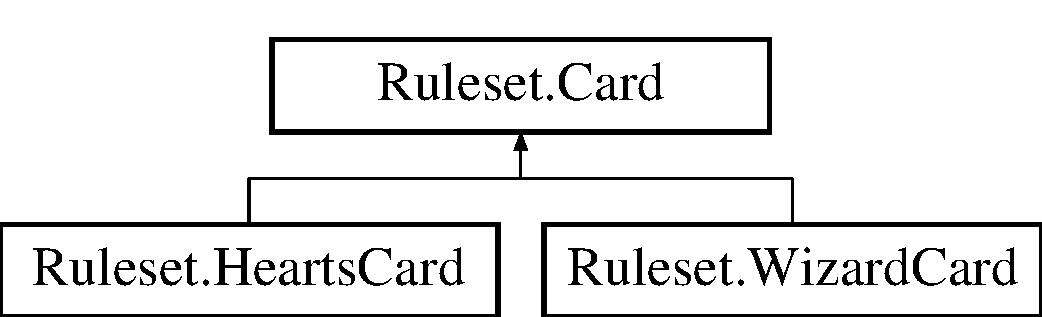
\includegraphics[height=3.000000cm]{a00001}
\end{center}
\end{figure}
\subsubsection*{Öffentliche Methoden}
\begin{DoxyCompactItemize}
\item 
\hyperlink{a00001_a97eccc3cbe788dd025fe0b8e75165181}{Card} (String s)
\end{DoxyCompactItemize}


\subsubsection{Ausführliche Beschreibung}
Sie wird verwendet um einzelne Karten auf das Spielfeld zu zeichnen. Dazu enthält sie die Pfadangabe zu dem Ordner, in dem die Bilder der Karten gespeichert sind, und eine I\-D, um das genaue Bild zu spezifizieren. 

\subsubsection{Beschreibung der Konstruktoren und Destruktoren}
\hypertarget{a00001_a97eccc3cbe788dd025fe0b8e75165181}{\index{Client\-::\-View\-::\-Card@{Client\-::\-View\-::\-Card}!Card@{Card}}
\index{Card@{Card}!Client::View::Card@{Client\-::\-View\-::\-Card}}
\paragraph[{Card}]{\setlength{\rightskip}{0pt plus 5cm}Client.\-View.\-Card.\-Card (
\begin{DoxyParamCaption}
\item[{String}]{s}
\end{DoxyParamCaption}
)}}\label{a00001_a97eccc3cbe788dd025fe0b8e75165181}


Erstellt eine neue Karte für die Anzeige und zeichnet dafür das Bild, das durch die Pfadangabe s angegeben ist. 


\begin{DoxyParams}{Parameter}
{\em s} & Pfadangabe zum zu zeichnenden Bild \\
\hline
\end{DoxyParams}

\hypertarget{a00002}{\subsection{Client\-Main Klassenreferenz}
\label{a00002}\index{Client\-Main@{Client\-Main}}
}
\subsubsection*{Öffentliche, statische Methoden}
\begin{DoxyCompactItemize}
\item 
static void \hyperlink{a00002_afd8ce3c47844bcb10ccd52d43dc4d339}{main} (final String\mbox{[}$\,$\mbox{]} args)
\end{DoxyCompactItemize}
\subsubsection*{Private Attribute}
\begin{DoxyCompactItemize}
\item 
\hypertarget{a00002_acb404ab350ff7496df1d66c7c638a7bd}{\hyperlink{a00001}{Client\-Controller} \hyperlink{a00002_acb404ab350ff7496df1d66c7c638a7bd}{client\-Controller}}\label{a00002_acb404ab350ff7496df1d66c7c638a7bd}

\end{DoxyCompactItemize}


\subsubsection{Ausführliche Beschreibung}
Die \hyperlink{a00002}{Client\-Main} Klasse startet den Spielclient und initialisiert dessen Komponenten. 

\subsubsection{Dokumentation der Elementfunktionen}
\hypertarget{a00002_afd8ce3c47844bcb10ccd52d43dc4d339}{\index{Client\-::\-Client\-Main@{Client\-::\-Client\-Main}!main@{main}}
\index{main@{main}!Client::ClientMain@{Client\-::\-Client\-Main}}
\paragraph[{main}]{\setlength{\rightskip}{0pt plus 5cm}static void main (
\begin{DoxyParamCaption}
\item[{final String\mbox{[}$\,$\mbox{]}}]{args}
\end{DoxyParamCaption}
)\hspace{0.3cm}{\ttfamily [static]}}}\label{a00002_afd8ce3c47844bcb10ccd52d43dc4d339}

\begin{DoxyParams}{Parameter}
{\em args} & \\
\hline
\end{DoxyParams}

\hypertarget{a00003}{\subsection{Ruleset.\-Card\-Deck Klassenreferenz}
\label{a00003}\index{Ruleset.\-Card\-Deck@{Ruleset.\-Card\-Deck}}
}

\hypertarget{a00004}{\subsection{Ruleset.\-Client\-Wizard Klassenreferenz}
\label{a00004}\index{Ruleset.\-Client\-Wizard@{Ruleset.\-Client\-Wizard}}
}
Klassendiagramm für Ruleset.\-Client\-Wizard\-:\begin{figure}[H]
\begin{center}
\leavevmode
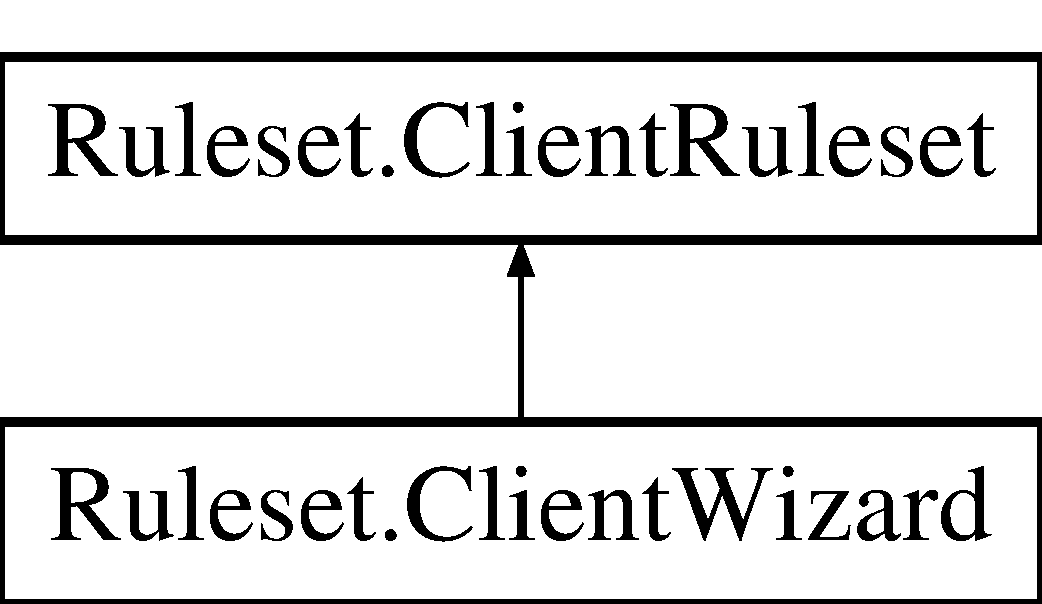
\includegraphics[height=2.000000cm]{a00004}
\end{center}
\end{figure}
\subsubsection*{Öffentliche Methoden}
\begin{DoxyCompactItemize}
\item 
boolean \hyperlink{a00004_a375a6aca8ba78551d0da0f6840cec6aa}{is\-Valid\-Move} (\hyperlink{a00001}{Card} card)
\end{DoxyCompactItemize}


\subsubsection{Ausführliche Beschreibung}
\begin{DoxyAuthor}{Autor}
m4nkey  \char`\"{}\-U\-M\-L to Java (com.\-ibm.\-xtools.\-transform.\-uml2.\-java5.\-internal.\-U\-M\-L2\-Java\-Transform)\char`\"{} 
\end{DoxyAuthor}


\subsubsection{Dokumentation der Elementfunktionen}
\hypertarget{a00004_a375a6aca8ba78551d0da0f6840cec6aa}{\index{Ruleset\-::\-Client\-Wizard@{Ruleset\-::\-Client\-Wizard}!is\-Valid\-Move@{is\-Valid\-Move}}
\index{is\-Valid\-Move@{is\-Valid\-Move}!Ruleset::ClientWizard@{Ruleset\-::\-Client\-Wizard}}
\paragraph[{is\-Valid\-Move}]{\setlength{\rightskip}{0pt plus 5cm}boolean Ruleset.\-Client\-Wizard.\-is\-Valid\-Move (
\begin{DoxyParamCaption}
\item[{{\bf Card}}]{card}
\end{DoxyParamCaption}
)\hspace{0.3cm}{\ttfamily [virtual]}}}\label{a00004_a375a6aca8ba78551d0da0f6840cec6aa}


Pr�ft ob ein gemachter Zug zum Spiel Wizard g�ltig ist. 

\begin{DoxyReturn}{Rückgabe}
is\-Valid true falls Zug g�ltig, false wenn nicht 
\end{DoxyReturn}


Implementiert \hyperlink{a00003_aa335aa62f13ac6ef532aef65a8cb34c0}{Ruleset.\-Client\-Ruleset}.


\hypertarget{a00005}{\subsection{Message\-Listener\-Thread Klassenreferenz}
\label{a00005}\index{Message\-Listener\-Thread@{Message\-Listener\-Thread}}
}


Abgeleitet von Thread.

\subsubsection*{Öffentliche Methoden}
\begin{DoxyCompactItemize}
\item 
\hypertarget{a00005_a90ebca0a8a2d843065708a4473f4428d}{\hyperlink{a00005_a90ebca0a8a2d843065708a4473f4428d}{Message\-Listener\-Thread} ()}\label{a00005_a90ebca0a8a2d843065708a4473f4428d}

\item 
void \hyperlink{a00005_a9b5e6f31c533ba11eada7bdd1767bf10}{start\-Connection} (\hyperlink{a00003}{Client\-Model} model, Socket connection)  throws Illegal\-Argument\-Exception, I\-O\-Exception 
\item 
\hypertarget{a00005_aaf912c696192e6a13eb70526891b4cd2}{void \hyperlink{a00005_aaf912c696192e6a13eb70526891b4cd2}{close\-Connection} ()}\label{a00005_aaf912c696192e6a13eb70526891b4cd2}

\item 
\hypertarget{a00005_afea035a8450d55661a10d4727154498d}{void \hyperlink{a00005_afea035a8450d55661a10d4727154498d}{send} (\hyperlink{a00037}{Com\-Object} object)}\label{a00005_afea035a8450d55661a10d4727154498d}

\item 
\hypertarget{a00005_a13a43e6d814de94978c515cb084873b1}{void \hyperlink{a00005_a13a43e6d814de94978c515cb084873b1}{run} ()}\label{a00005_a13a43e6d814de94978c515cb084873b1}

\end{DoxyCompactItemize}
\subsubsection*{Private Attribute}
\begin{DoxyCompactItemize}
\item 
\hypertarget{a00005_a5ea451c5997894ff409c7feb3ed28448}{Socket {\bfseries socket}}\label{a00005_a5ea451c5997894ff409c7feb3ed28448}

\item 
\hypertarget{a00005_af04a77f17fee54627c647f7d430fd7e4}{Object\-Input {\bfseries in}}\label{a00005_af04a77f17fee54627c647f7d430fd7e4}

\item 
\hypertarget{a00005_aaa47df5af3623385a32344b55b1aa173}{Object\-Output {\bfseries out}}\label{a00005_aaa47df5af3623385a32344b55b1aa173}

\item 
\hypertarget{a00005_acd2be1cfc258f9da5c30cf341d2a8804}{boolean {\bfseries run} = false}\label{a00005_acd2be1cfc258f9da5c30cf341d2a8804}

\item 
\hypertarget{a00005_a816de8cbcf19fd6762e3c5e5c66af478}{\hyperlink{a00003}{Client\-Model} {\bfseries model}}\label{a00005_a816de8cbcf19fd6762e3c5e5c66af478}

\end{DoxyCompactItemize}


\subsubsection{Ausführliche Beschreibung}
Diese Klasse implementiert die Netzwerkanbindung des Clients an den Server. Sie enthaelt den dazu noetigen Socket und Objekt\-Stream Reader und Writer. 

\subsubsection{Dokumentation der Elementfunktionen}
\hypertarget{a00005_a9b5e6f31c533ba11eada7bdd1767bf10}{\index{Client\-::\-Message\-Listener\-Thread@{Client\-::\-Message\-Listener\-Thread}!start\-Connection@{start\-Connection}}
\index{start\-Connection@{start\-Connection}!Client::MessageListenerThread@{Client\-::\-Message\-Listener\-Thread}}
\paragraph[{start\-Connection}]{\setlength{\rightskip}{0pt plus 5cm}void start\-Connection (
\begin{DoxyParamCaption}
\item[{{\bf Client\-Model}}]{model, }
\item[{Socket}]{connection}
\end{DoxyParamCaption}
) throws Illegal\-Argument\-Exception, I\-O\-Exception}}\label{a00005_a9b5e6f31c533ba11eada7bdd1767bf10}


Initialisiert die Object\-Streams und speichert den T\-C\-P Socket im Thread. 


\begin{DoxyParams}{Parameter}
{\em model} & \hyperlink{a00003}{Client\-Model}, Das Model das den Spielablauf und Serverkommunikation steuert. \\
\hline
{\em connection} & Socket, der Socket über den die T\-C\-P Verbindung laeuft. \\
\hline
\end{DoxyParams}

\begin{DoxyExceptions}{Ausnahmebehandlung}
{\em Illegal\-Argument\-Exception} & Wird geworfen bei falschen \hyperlink{a00003}{Client\-Model} oder Socket Argumenten. \\
\hline
{\em I\-O\-Exception} & Wird geworfen beim fehlerbehafteten Erstellen der Object\-Streams. \\
\hline
\end{DoxyExceptions}

\hypertarget{a00006}{\subsection{Choose\-Cards Klassenreferenz}
\label{a00006}\index{Choose\-Cards@{Choose\-Cards}}
}


Abgeleitet von Observer.

\subsubsection*{Öffentliche Methoden}
\begin{DoxyCompactItemize}
\item 
void \hyperlink{a00006_a2b67d42550fdf9ddd8f3878d0849965c}{update} (Observable o, Object arg)
\end{DoxyCompactItemize}
\subsubsection*{Private Attribute}
\begin{DoxyCompactItemize}
\item 
\hypertarget{a00006_a78a1f793ce7650a7cfefc4a7e4d14a04}{\hyperlink{a00019}{Own\-Hand} {\bfseries player\-Hand\-Panel}}\label{a00006_a78a1f793ce7650a7cfefc4a7e4d14a04}

\end{DoxyCompactItemize}


\subsubsection{Ausführliche Beschreibung}
In diesem Fenster muss der Benutzer eine vorbestimmte Menge Karten auswaehlen. 

\subsubsection{Dokumentation der Elementfunktionen}
\hypertarget{a00006_a2b67d42550fdf9ddd8f3878d0849965c}{\index{Client\-::\-View\-::\-Choose\-Cards@{Client\-::\-View\-::\-Choose\-Cards}!update@{update}}
\index{update@{update}!Client::View::ChooseCards@{Client\-::\-View\-::\-Choose\-Cards}}
\paragraph[{update}]{\setlength{\rightskip}{0pt plus 5cm}void update (
\begin{DoxyParamCaption}
\item[{Observable}]{o, }
\item[{Object}]{arg}
\end{DoxyParamCaption}
)}}\label{a00006_a2b67d42550fdf9ddd8f3878d0849965c}


Wird durch notify() im \hyperlink{a00003}{Client\-Model} aufgerufen. 

Je nach dem in arg uebergebenen Befehl wird ein Update des Fensters ausgefuehrt oder eine Fehlermeldung angezeigt.


\begin{DoxyParams}{Parameter}
{\em o} & erwartet ein Objekt von der Klasse \hyperlink{a00003}{Client\-Model} \\
\hline
{\em arg} & erwartet\-: open\-Choose\-Cards, choose\-Cards\-Successful \\
\hline
\end{DoxyParams}

\hypertarget{a00007}{\subsection{Choose\-Item Klassenreferenz}
\label{a00007}\index{Choose\-Item@{Choose\-Item}}
}


Abgeleitet von Observer.

\subsubsection*{Öffentliche Methoden}
\begin{DoxyCompactItemize}
\item 
void \hyperlink{a00007_a5e5bb525779faa05530c9ebdc49ad123}{update} (Observable arg0, Object arg1)
\end{DoxyCompactItemize}
\subsubsection*{Private Attribute}
\begin{DoxyCompactItemize}
\item 
\hypertarget{a00007_a5eae36bb5790864ced94623c9d08cb90}{Object {\bfseries item\-Combo\-Box}}\label{a00007_a5eae36bb5790864ced94623c9d08cb90}

\end{DoxyCompactItemize}


\subsubsection{Ausführliche Beschreibung}
Dieses Fenster ermoeglicht es dem Spieler aus einer Liste von Items eines auszuwaehlen. 

\subsubsection{Dokumentation der Elementfunktionen}
\hypertarget{a00007_a5e5bb525779faa05530c9ebdc49ad123}{\index{Client\-::\-View\-::\-Choose\-Item@{Client\-::\-View\-::\-Choose\-Item}!update@{update}}
\index{update@{update}!Client::View::ChooseItem@{Client\-::\-View\-::\-Choose\-Item}}
\paragraph[{update}]{\setlength{\rightskip}{0pt plus 5cm}void update (
\begin{DoxyParamCaption}
\item[{Observable}]{arg0, }
\item[{Object}]{arg1}
\end{DoxyParamCaption}
)}}\label{a00007_a5e5bb525779faa05530c9ebdc49ad123}


Wird durch notify() im \hyperlink{a00003}{Client\-Model} aufgerufen. 

Je nach dem in arg uebergebenen Befehl wird ein Update des Fensters ausgefuehrt oder eine Fehlermeldung angezeigt.


\begin{DoxyParams}{Parameter}
{\em o} & erwartet ein Objekt von der Klasse \hyperlink{a00003}{Client\-Model} \\
\hline
{\em arg} & erwartet\-: open\-Choose\-Item, choose\-Item\-Successful \\
\hline
\end{DoxyParams}

\hypertarget{a00008}{\subsection{Create\-Game Klassenreferenz}
\label{a00008}\index{Create\-Game@{Create\-Game}}
}


Abgeleitet von J\-Frame.

\subsubsection*{Öffentliche Methoden}
\begin{DoxyCompactItemize}
\item 
\hypertarget{a00008_a9c81ed380a56f523fd8a7b0c8fc349f7}{\hyperlink{a00008_a9c81ed380a56f523fd8a7b0c8fc349f7}{Create\-Game} ()}\label{a00008_a9c81ed380a56f523fd8a7b0c8fc349f7}

\item 
void \hyperlink{a00008_a0e4f14000bb92efe86644965867a5156}{add\-Panel\-Mouse\-Listener} (Mouse\-Listener m)
\item 
void \hyperlink{a00008_acf3b22c2ad67e52fbd300665503a0cb5}{add\-Ruleset\-Selection\-Listener} (Item\-Listener i)
\item 
void \hyperlink{a00008_a766141ddea860fac0deb3ceb1c65ed60}{add\-Create\-Button\-Listener} (Action\-Listener a)
\item 
void \hyperlink{a00008_aac8c97a2425ab3702a82bb0876aa3cc8}{add\-Leave\-Button\-Listener} (Action\-Listener a)
\item 
void \hyperlink{a00008_a9329ba7453dd661d50d2fb8024df3b2b}{set\-Language} (\hyperlink{a00015}{Language} l)
\end{DoxyCompactItemize}
\subsubsection*{Öffentliche, statische Methoden}
\begin{DoxyCompactItemize}
\item 
\hypertarget{a00008_a8b260eecbaabcef8473fd87ada040682}{static void {\bfseries main} (String\mbox{[}$\,$\mbox{]} args)}\label{a00008_a8b260eecbaabcef8473fd87ada040682}

\end{DoxyCompactItemize}
\subsubsection*{Private Methoden}
\begin{DoxyCompactItemize}
\item 
\hypertarget{a00008_a74cba330cee84fa07487e12fdafe29aa}{void {\bfseries update\-Language} ()}\label{a00008_a74cba330cee84fa07487e12fdafe29aa}

\end{DoxyCompactItemize}
\subsubsection*{Private Attribute}
\begin{DoxyCompactItemize}
\item 
\hypertarget{a00008_a430764470b3602491655161cdd67ee8c}{\hyperlink{a00015}{Language} {\bfseries lang}}\label{a00008_a430764470b3602491655161cdd67ee8c}

\item 
\hypertarget{a00008_a2b4470f7f3f7456c7e52d1604438a878}{J\-Text\-Field {\bfseries name\-Field}}\label{a00008_a2b4470f7f3f7456c7e52d1604438a878}

\item 
\hypertarget{a00008_a45e94f786577439d02e4f16aefa96717}{Buffered\-Image {\bfseries image}}\label{a00008_a45e94f786577439d02e4f16aefa96717}

\item 
\hypertarget{a00008_ab86817c3677c2dc422445fe8c0b5a404}{J\-Text\-Field {\bfseries password\-Field}}\label{a00008_ab86817c3677c2dc422445fe8c0b5a404}

\item 
\hypertarget{a00008_a8f4aaa528d2092952844a99aa948932f}{J\-Panel {\bfseries image\-Panel}}\label{a00008_a8f4aaa528d2092952844a99aa948932f}

\item 
\hypertarget{a00008_ac3a56e854d86f838fbfe3bad5fca49ea}{J\-Label {\bfseries lbl\-Select}}\label{a00008_ac3a56e854d86f838fbfe3bad5fca49ea}

\item 
\hypertarget{a00008_a7916a564649b0412714b6ea8c2251812}{J\-Combo\-Box$<$ String $>$ {\bfseries ruleset\-Box}}\label{a00008_a7916a564649b0412714b6ea8c2251812}

\item 
\hypertarget{a00008_a5df88a40b8ff9b13b83ca12563ba89c7}{J\-Check\-Box {\bfseries chckbx\-Password}}\label{a00008_a5df88a40b8ff9b13b83ca12563ba89c7}

\item 
\hypertarget{a00008_a1887f14b78aa91b00e5ce42aa504dbe2}{J\-Button {\bfseries btn\-Leave}}\label{a00008_a1887f14b78aa91b00e5ce42aa504dbe2}

\item 
\hypertarget{a00008_a69446706c0a5c7165a4de4f64d7b2261}{J\-Button {\bfseries btn\-Create}}\label{a00008_a69446706c0a5c7165a4de4f64d7b2261}

\item 
\hypertarget{a00008_a59c71155f1fd33a521bce1afebc0863b}{J\-Label {\bfseries lbl\-Game\-Name}}\label{a00008_a59c71155f1fd33a521bce1afebc0863b}

\end{DoxyCompactItemize}
\subsubsection*{Statische, private Attribute}
\begin{DoxyCompactItemize}
\item 
\hypertarget{a00008_a3238d314ecdee14d2966760945d00c3b}{static final long {\bfseries serial\-Version\-U\-I\-D} = -\/2893031560688870723\-L}\label{a00008_a3238d314ecdee14d2966760945d00c3b}

\end{DoxyCompactItemize}


\subsubsection{Ausführliche Beschreibung}
Das Fenster \hyperlink{a00008}{Create\-Game} dient dem Benutzer zur Erstellung eines neuen Spieles. Es bietet alle Komponenten, um ein Regelwerk zu waehlen, einen Spielnamen festzulegen und das Spiel durch ein Passwort zu schuetzen. In der Spielerstellung wird ein Titelbild des ausgewaehlten Spiels und eine kurze Beschreibung angezeigt. ueber 'Leave' kehrt der Spieler in die \hyperlink{a00016}{Lobby} zurueck und mit 'Create' wird das Spiel erstellt. 

\subsubsection{Dokumentation der Elementfunktionen}
\hypertarget{a00008_a0e4f14000bb92efe86644965867a5156}{\index{Client\-::\-View\-::\-Create\-Game@{Client\-::\-View\-::\-Create\-Game}!add\-Panel\-Mouse\-Listener@{add\-Panel\-Mouse\-Listener}}
\index{add\-Panel\-Mouse\-Listener@{add\-Panel\-Mouse\-Listener}!Client::View::CreateGame@{Client\-::\-View\-::\-Create\-Game}}
\paragraph[{add\-Panel\-Mouse\-Listener}]{\setlength{\rightskip}{0pt plus 5cm}void add\-Panel\-Mouse\-Listener (
\begin{DoxyParamCaption}
\item[{Mouse\-Listener}]{m}
\end{DoxyParamCaption}
)}}\label{a00008_a0e4f14000bb92efe86644965867a5156}


Fuegt einen Mouse\-Listener zum Image\-Panel des \hyperlink{a00008}{Create\-Game} Fensters hinzu, der zur Anzeige des Mouse\-Over-\/\-Texts verwendet wird. 


\begin{DoxyParams}{Parameter}
{\em m} & ein Mouse\-Listener \\
\hline
\end{DoxyParams}
\hypertarget{a00008_acf3b22c2ad67e52fbd300665503a0cb5}{\index{Client\-::\-View\-::\-Create\-Game@{Client\-::\-View\-::\-Create\-Game}!add\-Ruleset\-Selection\-Listener@{add\-Ruleset\-Selection\-Listener}}
\index{add\-Ruleset\-Selection\-Listener@{add\-Ruleset\-Selection\-Listener}!Client::View::CreateGame@{Client\-::\-View\-::\-Create\-Game}}
\paragraph[{add\-Ruleset\-Selection\-Listener}]{\setlength{\rightskip}{0pt plus 5cm}void add\-Ruleset\-Selection\-Listener (
\begin{DoxyParamCaption}
\item[{Item\-Listener}]{i}
\end{DoxyParamCaption}
)}}\label{a00008_acf3b22c2ad67e52fbd300665503a0cb5}


Fuegt einen Listener fuer die Regelwerk-\/\-Auswahl des \hyperlink{a00008}{Create\-Game} Fensters hinzu. 


\begin{DoxyParams}{Parameter}
{\em i} & ein Item\-Listener \\
\hline
\end{DoxyParams}
\hypertarget{a00008_a766141ddea860fac0deb3ceb1c65ed60}{\index{Client\-::\-View\-::\-Create\-Game@{Client\-::\-View\-::\-Create\-Game}!add\-Create\-Button\-Listener@{add\-Create\-Button\-Listener}}
\index{add\-Create\-Button\-Listener@{add\-Create\-Button\-Listener}!Client::View::CreateGame@{Client\-::\-View\-::\-Create\-Game}}
\paragraph[{add\-Create\-Button\-Listener}]{\setlength{\rightskip}{0pt plus 5cm}void add\-Create\-Button\-Listener (
\begin{DoxyParamCaption}
\item[{Action\-Listener}]{a}
\end{DoxyParamCaption}
)}}\label{a00008_a766141ddea860fac0deb3ceb1c65ed60}


Fuegt einen Action\-Listener fuer den 'Create' Button hinzu. 


\begin{DoxyParams}{Parameter}
{\em a} & ein Action\-Listener \\
\hline
\end{DoxyParams}
\hypertarget{a00008_aac8c97a2425ab3702a82bb0876aa3cc8}{\index{Client\-::\-View\-::\-Create\-Game@{Client\-::\-View\-::\-Create\-Game}!add\-Leave\-Button\-Listener@{add\-Leave\-Button\-Listener}}
\index{add\-Leave\-Button\-Listener@{add\-Leave\-Button\-Listener}!Client::View::CreateGame@{Client\-::\-View\-::\-Create\-Game}}
\paragraph[{add\-Leave\-Button\-Listener}]{\setlength{\rightskip}{0pt plus 5cm}void add\-Leave\-Button\-Listener (
\begin{DoxyParamCaption}
\item[{Action\-Listener}]{a}
\end{DoxyParamCaption}
)}}\label{a00008_aac8c97a2425ab3702a82bb0876aa3cc8}


Fuegt einen Action\-Listener fuer den 'Leave' Button hinzu. 


\begin{DoxyParams}{Parameter}
{\em a} & ein Action\-Listener \\
\hline
\end{DoxyParams}
\hypertarget{a00008_a9329ba7453dd661d50d2fb8024df3b2b}{\index{Client\-::\-View\-::\-Create\-Game@{Client\-::\-View\-::\-Create\-Game}!set\-Language@{set\-Language}}
\index{set\-Language@{set\-Language}!Client::View::CreateGame@{Client\-::\-View\-::\-Create\-Game}}
\paragraph[{set\-Language}]{\setlength{\rightskip}{0pt plus 5cm}void set\-Language (
\begin{DoxyParamCaption}
\item[{{\bf Language}}]{l}
\end{DoxyParamCaption}
)}}\label{a00008_a9329ba7453dd661d50d2fb8024df3b2b}


Aendert die Sprache des Fensters. 


\begin{DoxyParams}{Parameter}
{\em l} & Sprache in Form des Language-\/\-Enums \\
\hline
\end{DoxyParams}

\hypertarget{a00009}{\subsection{Discard\-Pile Klassenreferenz}
\label{a00009}\index{Discard\-Pile@{Discard\-Pile}}
}
\subsubsection*{Private Attribute}
\begin{DoxyCompactItemize}
\item 
\hypertarget{a00009_a32963d9bbf9a4ad1ca8d0e1cf6c54bfe}{Set$<$ \hyperlink{a00022}{View\-Card} $>$ {\bfseries card}}\label{a00009_a32963d9bbf9a4ad1ca8d0e1cf6c54bfe}

\end{DoxyCompactItemize}


\subsubsection{Ausführliche Beschreibung}
Stellt einen Ablagestapel dar, dieser kann sowohl für jeden Spieler einzeln oder für alle Spieler gemeinsam in der Mitte des Spielfeldes angezeigt werden. 
\hypertarget{a00010}{\subsection{Draw\-Deck Klassenreferenz}
\label{a00010}\index{Draw\-Deck@{Draw\-Deck}}
}


\subsubsection{Ausführliche Beschreibung}
Stellt einen Aufnahmestapel dar. 
\hypertarget{a00011}{\subsection{Server.\-Lobby\-Server.\-Client\-Listener\-Thread Klassenreferenz}
\label{a00011}\index{Server.\-Lobby\-Server.\-Client\-Listener\-Thread@{Server.\-Lobby\-Server.\-Client\-Listener\-Thread}}
}
Klassendiagramm für Server.\-Lobby\-Server.\-Client\-Listener\-Thread\-:\begin{figure}[H]
\begin{center}
\leavevmode
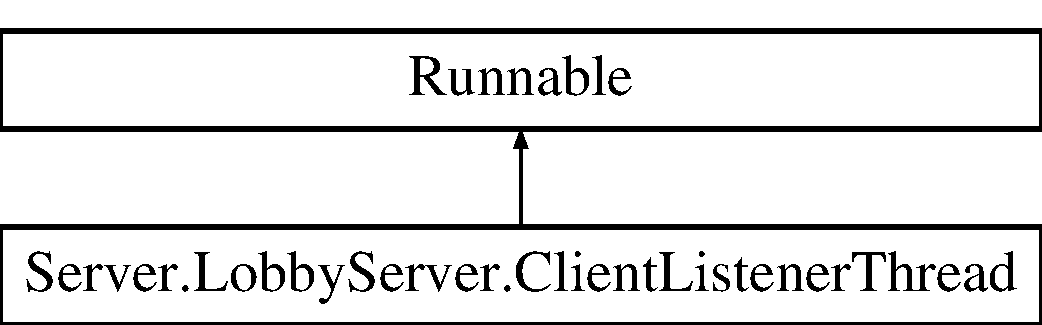
\includegraphics[height=2.000000cm]{a00011}
\end{center}
\end{figure}


\subsubsection{Ausführliche Beschreibung}
Der Thread auf eingehende Clientverbindungen, stellt diese her und instanziiert für jede Verbindung eine Klasse \hyperlink{a00073}{Player}. Dieser wird dann dem \hyperlink{a00054}{Lobby\-Server} übergeben. \begin{DoxyAuthor}{Autor}
Viktoria 
\end{DoxyAuthor}

\hypertarget{a00012}{\subsection{Game\-Lobby Klassenreferenz}
\label{a00012}\index{Game\-Lobby@{Game\-Lobby}}
}


Abgeleitet von J\-Frame und Observer.

\subsubsection*{Öffentliche Methoden}
\begin{DoxyCompactItemize}
\item 
\hypertarget{a00012_af5c160b3c4448522e0d6e0002470c80e}{\hyperlink{a00012_af5c160b3c4448522e0d6e0002470c80e}{Game\-Lobby} ()}\label{a00012_af5c160b3c4448522e0d6e0002470c80e}

\item 
void \hyperlink{a00012_a865971050de64d103900e70b236a0b92}{add\-Start\-Button\-Listener} (Action\-Listener a)
\item 
void \hyperlink{a00012_ab66ade112f82eb29655a140d34bae4fd}{add\-Remove\-Button\-Listener} (Action\-Listener a)
\item 
void \hyperlink{a00012_aac8c97a2425ab3702a82bb0876aa3cc8}{add\-Leave\-Button\-Listener} (Action\-Listener a)
\item 
void \hyperlink{a00012_a1d0d058b74950bbf7305be79b1d60143}{add\-Chat\-Message\-Listener} (Key\-Listener k)
\item 
void \hyperlink{a00012_a9329ba7453dd661d50d2fb8024df3b2b}{set\-Language} (\hyperlink{a00015}{Language} l)
\item 
void \hyperlink{a00012_a2b67d42550fdf9ddd8f3878d0849965c}{update} (Observable o, Object arg)
\item 
void \hyperlink{a00012_a41caffb40957934b02960cf166c78494}{update} (Observable o, String arg)
\end{DoxyCompactItemize}
\subsubsection*{Öffentliche, statische Methoden}
\begin{DoxyCompactItemize}
\item 
\hypertarget{a00012_a8b260eecbaabcef8473fd87ada040682}{static void {\bfseries main} (String\mbox{[}$\,$\mbox{]} args)}\label{a00012_a8b260eecbaabcef8473fd87ada040682}

\end{DoxyCompactItemize}
\subsubsection*{Private Methoden}
\begin{DoxyCompactItemize}
\item 
\hypertarget{a00012_a74cba330cee84fa07487e12fdafe29aa}{void {\bfseries update\-Language} ()}\label{a00012_a74cba330cee84fa07487e12fdafe29aa}

\end{DoxyCompactItemize}
\subsubsection*{Private Attribute}
\begin{DoxyCompactItemize}
\item 
\hypertarget{a00012_aee369a2eca6b8f16ea106cddf68273e8}{J\-Panel {\bfseries content\-Pane}}\label{a00012_aee369a2eca6b8f16ea106cddf68273e8}

\item 
\hypertarget{a00012_aeaa6444a9657e78f8c42051d5f7b4ff6}{J\-Text\-Field {\bfseries message\-Field}}\label{a00012_aeaa6444a9657e78f8c42051d5f7b4ff6}

\item 
\hypertarget{a00012_a430764470b3602491655161cdd67ee8c}{\hyperlink{a00015}{Language} {\bfseries lang}}\label{a00012_a430764470b3602491655161cdd67ee8c}

\item 
\hypertarget{a00012_ad9e9e9e7b8ce2d427def6cc55ef526bd}{J\-Button {\bfseries btn\-Remove\-Player}}\label{a00012_ad9e9e9e7b8ce2d427def6cc55ef526bd}

\item 
\hypertarget{a00012_a1887f14b78aa91b00e5ce42aa504dbe2}{J\-Button {\bfseries btn\-Leave}}\label{a00012_a1887f14b78aa91b00e5ce42aa504dbe2}

\item 
\hypertarget{a00012_a12e216d7d1a56c6e799be1f874c7c82c}{J\-Text\-Area {\bfseries chatlog}}\label{a00012_a12e216d7d1a56c6e799be1f874c7c82c}

\item 
\hypertarget{a00012_a1ac11a30aed65ffc1a336a48515ea9de}{J\-Button {\bfseries btn\-Start\-Game}}\label{a00012_a1ac11a30aed65ffc1a336a48515ea9de}

\end{DoxyCompactItemize}
\subsubsection*{Statische, private Attribute}
\begin{DoxyCompactItemize}
\item 
\hypertarget{a00012_a3238d314ecdee14d2966760945d00c3b}{static final long {\bfseries serial\-Version\-U\-I\-D} = -\/1899311213351027436\-L}\label{a00012_a3238d314ecdee14d2966760945d00c3b}

\end{DoxyCompactItemize}


\subsubsection{Ausführliche Beschreibung}
Die \hyperlink{a00012}{Game\-Lobby} modelliert das Wartefenster, in dem beigetretene Spieler auf den Start des Spieles durch den Spielleiter warten. Der Spielleiter kann Spieler mit dem Remove Player Button entfernen. ueber Leave kehren die Spieler in die \hyperlink{a00016}{Lobby} zurueck. Der spielinterne Chat ist ab hier verfuegbar. 

\subsubsection{Dokumentation der Elementfunktionen}
\hypertarget{a00012_a865971050de64d103900e70b236a0b92}{\index{Client\-::\-View\-::\-Game\-Lobby@{Client\-::\-View\-::\-Game\-Lobby}!add\-Start\-Button\-Listener@{add\-Start\-Button\-Listener}}
\index{add\-Start\-Button\-Listener@{add\-Start\-Button\-Listener}!Client::View::GameLobby@{Client\-::\-View\-::\-Game\-Lobby}}
\paragraph[{add\-Start\-Button\-Listener}]{\setlength{\rightskip}{0pt plus 5cm}void add\-Start\-Button\-Listener (
\begin{DoxyParamCaption}
\item[{Action\-Listener}]{a}
\end{DoxyParamCaption}
)}}\label{a00012_a865971050de64d103900e70b236a0b92}


Fuegt einen Action\-Listener fuer den 'Start \hyperlink{a00011}{Game}' Button hinzu. 


\begin{DoxyParams}{Parameter}
{\em a} & ein Action\-Listener \\
\hline
\end{DoxyParams}
\hypertarget{a00012_ab66ade112f82eb29655a140d34bae4fd}{\index{Client\-::\-View\-::\-Game\-Lobby@{Client\-::\-View\-::\-Game\-Lobby}!add\-Remove\-Button\-Listener@{add\-Remove\-Button\-Listener}}
\index{add\-Remove\-Button\-Listener@{add\-Remove\-Button\-Listener}!Client::View::GameLobby@{Client\-::\-View\-::\-Game\-Lobby}}
\paragraph[{add\-Remove\-Button\-Listener}]{\setlength{\rightskip}{0pt plus 5cm}void add\-Remove\-Button\-Listener (
\begin{DoxyParamCaption}
\item[{Action\-Listener}]{a}
\end{DoxyParamCaption}
)}}\label{a00012_ab66ade112f82eb29655a140d34bae4fd}


Fuegt einen Action\-Listener fuer den 'Remove Player' Button hinzu. 


\begin{DoxyParams}{Parameter}
{\em a} & ein Action\-Listener \\
\hline
\end{DoxyParams}
\hypertarget{a00012_aac8c97a2425ab3702a82bb0876aa3cc8}{\index{Client\-::\-View\-::\-Game\-Lobby@{Client\-::\-View\-::\-Game\-Lobby}!add\-Leave\-Button\-Listener@{add\-Leave\-Button\-Listener}}
\index{add\-Leave\-Button\-Listener@{add\-Leave\-Button\-Listener}!Client::View::GameLobby@{Client\-::\-View\-::\-Game\-Lobby}}
\paragraph[{add\-Leave\-Button\-Listener}]{\setlength{\rightskip}{0pt plus 5cm}void add\-Leave\-Button\-Listener (
\begin{DoxyParamCaption}
\item[{Action\-Listener}]{a}
\end{DoxyParamCaption}
)}}\label{a00012_aac8c97a2425ab3702a82bb0876aa3cc8}


Fuegt einen Action\-Listener fuer den 'Leave' Button hinzu. 


\begin{DoxyParams}{Parameter}
{\em a} & ein Action\-Listener \\
\hline
\end{DoxyParams}
\hypertarget{a00012_a1d0d058b74950bbf7305be79b1d60143}{\index{Client\-::\-View\-::\-Game\-Lobby@{Client\-::\-View\-::\-Game\-Lobby}!add\-Chat\-Message\-Listener@{add\-Chat\-Message\-Listener}}
\index{add\-Chat\-Message\-Listener@{add\-Chat\-Message\-Listener}!Client::View::GameLobby@{Client\-::\-View\-::\-Game\-Lobby}}
\paragraph[{add\-Chat\-Message\-Listener}]{\setlength{\rightskip}{0pt plus 5cm}void add\-Chat\-Message\-Listener (
\begin{DoxyParamCaption}
\item[{Key\-Listener}]{k}
\end{DoxyParamCaption}
)}}\label{a00012_a1d0d058b74950bbf7305be79b1d60143}


Fuet einen Key\-Listener fuer das Nachricht-\/\-Senden-\/\-Feld der \hyperlink{a00016}{Lobby} hinzu. 


\begin{DoxyParams}{Parameter}
{\em k} & \\
\hline
\end{DoxyParams}
\hypertarget{a00012_a9329ba7453dd661d50d2fb8024df3b2b}{\index{Client\-::\-View\-::\-Game\-Lobby@{Client\-::\-View\-::\-Game\-Lobby}!set\-Language@{set\-Language}}
\index{set\-Language@{set\-Language}!Client::View::GameLobby@{Client\-::\-View\-::\-Game\-Lobby}}
\paragraph[{set\-Language}]{\setlength{\rightskip}{0pt plus 5cm}void set\-Language (
\begin{DoxyParamCaption}
\item[{{\bf Language}}]{l}
\end{DoxyParamCaption}
)}}\label{a00012_a9329ba7453dd661d50d2fb8024df3b2b}


Aendert die Sprache des Fensters. 


\begin{DoxyParams}{Parameter}
{\em l} & Sprache in Form des Language-\/\-Enums \\
\hline
\end{DoxyParams}
\hypertarget{a00012_a2b67d42550fdf9ddd8f3878d0849965c}{\index{Client\-::\-View\-::\-Game\-Lobby@{Client\-::\-View\-::\-Game\-Lobby}!update@{update}}
\index{update@{update}!Client::View::GameLobby@{Client\-::\-View\-::\-Game\-Lobby}}
\paragraph[{update}]{\setlength{\rightskip}{0pt plus 5cm}void update (
\begin{DoxyParamCaption}
\item[{Observable}]{o, }
\item[{Object}]{arg}
\end{DoxyParamCaption}
)}}\label{a00012_a2b67d42550fdf9ddd8f3878d0849965c}


Wird durch notify() im \hyperlink{a00003}{Client\-Model} aufgerufen. 

Je nach dem in arg uebergebenen View\-Notification-\/\-Befehl wird ein Update des Fensters ausgefuehrt oder eine Fehlermeldung angezeigt.


\begin{DoxyParams}{Parameter}
{\em o} & erwartet ein Objekt von der Klasse \hyperlink{a00003}{Client\-Model} \\
\hline
{\em arg} & erwartet\-: join\-Game\-Successful, player\-List\-Update, window\-Change\-Forced, game\-Started \\
\hline
\end{DoxyParams}
\hypertarget{a00012_a41caffb40957934b02960cf166c78494}{\index{Client\-::\-View\-::\-Game\-Lobby@{Client\-::\-View\-::\-Game\-Lobby}!update@{update}}
\index{update@{update}!Client::View::GameLobby@{Client\-::\-View\-::\-Game\-Lobby}}
\paragraph[{update}]{\setlength{\rightskip}{0pt plus 5cm}void update (
\begin{DoxyParamCaption}
\item[{Observable}]{o, }
\item[{String}]{arg}
\end{DoxyParamCaption}
)}}\label{a00012_a41caffb40957934b02960cf166c78494}


Wird aufgerufen, wenn eine String-\/\-Nachricht im notify() uebergeben wird. 

Dieser wird als Chatnachricht interpretiert und dem Chatlog angefuegt.


\begin{DoxyParams}{Parameter}
{\em o} & erwartet ein Objekt von der Klasse \hyperlink{a00003}{Client\-Model} \\
\hline
{\em arg} & erwartet einen String, der eine Chatnachricht darstellt \\
\hline
\end{DoxyParams}

\hypertarget{a00013}{\subsection{Ruleset.\-Player\-State Klassenreferenz}
\label{a00013}\index{Ruleset.\-Player\-State@{Ruleset.\-Player\-State}}
}
\subsubsection*{Öffentliche Methoden}
\begin{DoxyCompactItemize}
\item 
String \hyperlink{a00013_a20076c230bb4bfa3404b53bead5194d7}{get\-Name} ()
\item 
Set$<$ \hyperlink{a00001}{Card} $>$ \hyperlink{a00013_ad95ba05e06f70d0ff6f774c3ae1b72b1}{get\-Hand} ()
\item 
\hyperlink{a00012}{Other\-Data} \hyperlink{a00013_ad913d4462ff4019b1d85ba534a27250e}{get\-Other\-Data} ()
\item 
void \hyperlink{a00013_a613eaeb717801aca760df6776d34d228}{add\-Card} (\hyperlink{a00001}{Card} card)
\item 
void \hyperlink{a00013_a38c66bb85292eaedd970cb1c6bc38dca}{remove\-Card} (\hyperlink{a00001}{Card} card)
\end{DoxyCompactItemize}


\subsubsection{Dokumentation der Elementfunktionen}
\hypertarget{a00013_a613eaeb717801aca760df6776d34d228}{\index{Ruleset\-::\-Player\-State@{Ruleset\-::\-Player\-State}!add\-Card@{add\-Card}}
\index{add\-Card@{add\-Card}!Ruleset::PlayerState@{Ruleset\-::\-Player\-State}}
\paragraph[{add\-Card}]{\setlength{\rightskip}{0pt plus 5cm}void Ruleset.\-Player\-State.\-add\-Card (
\begin{DoxyParamCaption}
\item[{{\bf Card}}]{card}
\end{DoxyParamCaption}
)}}\label{a00013_a613eaeb717801aca760df6776d34d228}


Gibt dem Spieler eine Karte. 


\begin{DoxyParams}{Parameter}
{\em card} & Die Karte die dem Spieler gegeben wird \\
\hline
\end{DoxyParams}
\hypertarget{a00013_ad95ba05e06f70d0ff6f774c3ae1b72b1}{\index{Ruleset\-::\-Player\-State@{Ruleset\-::\-Player\-State}!get\-Hand@{get\-Hand}}
\index{get\-Hand@{get\-Hand}!Ruleset::PlayerState@{Ruleset\-::\-Player\-State}}
\paragraph[{get\-Hand}]{\setlength{\rightskip}{0pt plus 5cm}Set$<${\bf Card}$>$ Ruleset.\-Player\-State.\-get\-Hand (
\begin{DoxyParamCaption}
{}
\end{DoxyParamCaption}
)}}\label{a00013_ad95ba05e06f70d0ff6f774c3ae1b72b1}


Holt die Kartenhand des Spielers. 

\begin{DoxyReturn}{Rückgabe}
own\-Hand Die Kartenhand des Spielers 
\end{DoxyReturn}
\hypertarget{a00013_a20076c230bb4bfa3404b53bead5194d7}{\index{Ruleset\-::\-Player\-State@{Ruleset\-::\-Player\-State}!get\-Name@{get\-Name}}
\index{get\-Name@{get\-Name}!Ruleset::PlayerState@{Ruleset\-::\-Player\-State}}
\paragraph[{get\-Name}]{\setlength{\rightskip}{0pt plus 5cm}String Ruleset.\-Player\-State.\-get\-Name (
\begin{DoxyParamCaption}
{}
\end{DoxyParamCaption}
)}}\label{a00013_a20076c230bb4bfa3404b53bead5194d7}


Holt den namen eines Spielers. 

\begin{DoxyReturn}{Rückgabe}
name Der Name des Spielers 
\end{DoxyReturn}
\hypertarget{a00013_ad913d4462ff4019b1d85ba534a27250e}{\index{Ruleset\-::\-Player\-State@{Ruleset\-::\-Player\-State}!get\-Other\-Data@{get\-Other\-Data}}
\index{get\-Other\-Data@{get\-Other\-Data}!Ruleset::PlayerState@{Ruleset\-::\-Player\-State}}
\paragraph[{get\-Other\-Data}]{\setlength{\rightskip}{0pt plus 5cm}{\bf Other\-Data} Ruleset.\-Player\-State.\-get\-Other\-Data (
\begin{DoxyParamCaption}
{}
\end{DoxyParamCaption}
)}}\label{a00013_ad913d4462ff4019b1d85ba534a27250e}


Holt die zus�tzlichen Informationen des Spielers. 

\begin{DoxyReturn}{Rückgabe}
own\-Hand Die zus�tzlichen Informationen des Spielers 
\end{DoxyReturn}
\hypertarget{a00013_a38c66bb85292eaedd970cb1c6bc38dca}{\index{Ruleset\-::\-Player\-State@{Ruleset\-::\-Player\-State}!remove\-Card@{remove\-Card}}
\index{remove\-Card@{remove\-Card}!Ruleset::PlayerState@{Ruleset\-::\-Player\-State}}
\paragraph[{remove\-Card}]{\setlength{\rightskip}{0pt plus 5cm}void Ruleset.\-Player\-State.\-remove\-Card (
\begin{DoxyParamCaption}
\item[{{\bf Card}}]{card}
\end{DoxyParamCaption}
)}}\label{a00013_a38c66bb85292eaedd970cb1c6bc38dca}


Entfernt eine Karte aus der Hand des Spielers. 


\begin{DoxyParams}{Parameter}
{\em card} & \\
\hline
\end{DoxyParams}

\hypertarget{a00014}{\subsection{Input\-Number Klassenreferenz}
\label{a00014}\index{Input\-Number@{Input\-Number}}
}


Abgeleitet von Observer.

\subsubsection*{Öffentliche Methoden}
\begin{DoxyCompactItemize}
\item 
void \hyperlink{a00014_a2b67d42550fdf9ddd8f3878d0849965c}{update} (Observable o, Object arg)
\end{DoxyCompactItemize}
\subsubsection*{Private Attribute}
\begin{DoxyCompactItemize}
\item 
\hypertarget{a00014_a6d8bcbe4ebb8e887e3dccb18c9ce3ad7}{Object {\bfseries number\-Textfield}}\label{a00014_a6d8bcbe4ebb8e887e3dccb18c9ce3ad7}

\end{DoxyCompactItemize}


\subsubsection{Ausführliche Beschreibung}
In diesem Fenster, kann der Benutzer eine Zahl eingeben. 

\subsubsection{Dokumentation der Elementfunktionen}
\hypertarget{a00014_a2b67d42550fdf9ddd8f3878d0849965c}{\index{Client\-::\-View\-::\-Input\-Number@{Client\-::\-View\-::\-Input\-Number}!update@{update}}
\index{update@{update}!Client::View::InputNumber@{Client\-::\-View\-::\-Input\-Number}}
\paragraph[{update}]{\setlength{\rightskip}{0pt plus 5cm}void update (
\begin{DoxyParamCaption}
\item[{Observable}]{o, }
\item[{Object}]{arg}
\end{DoxyParamCaption}
)}}\label{a00014_a2b67d42550fdf9ddd8f3878d0849965c}


Wird durch notify() im \hyperlink{a00003}{Client\-Model} aufgerufen. 

Je nach dem in arg uebergebenen Befehl wird ein Update des Fensters ausgefuehrt oder eine Fehlermeldung angezeigt.


\begin{DoxyParams}{Parameter}
{\em o} & erwartet ein Objekt von der Klasse \hyperlink{a00003}{Client\-Model} \\
\hline
{\em arg} & erwartet\-: open\-Input\-Number, input\-Number\-Successful \\
\hline
\end{DoxyParams}

\hypertarget{a00015}{\subsection{Client.\-Client\-State Enum-\/\-Referenz}
\label{a00015}\index{Client.\-Client\-State@{Client.\-Client\-State}}
}

\hypertarget{a00016}{\subsection{Ruleset.\-Server\-Ruleset Klassenreferenz}
\label{a00016}\index{Ruleset.\-Server\-Ruleset@{Ruleset.\-Server\-Ruleset}}
}
Klassendiagramm für Ruleset.\-Server\-Ruleset\-:\begin{figure}[H]
\begin{center}
\leavevmode
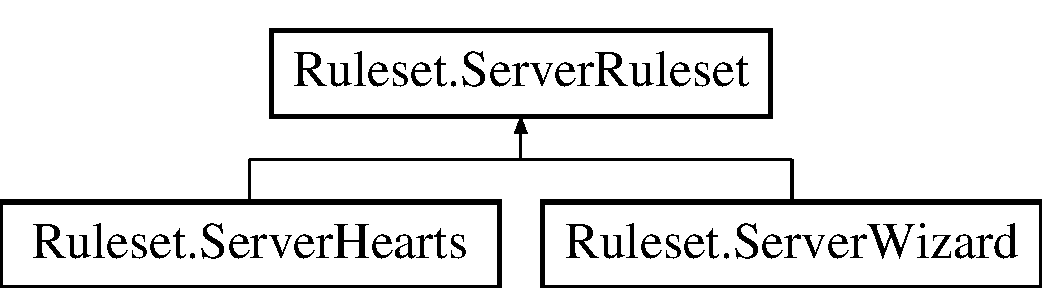
\includegraphics[height=2.000000cm]{a00016}
\end{center}
\end{figure}
\subsubsection*{Öffentliche Methoden}
\begin{DoxyCompactItemize}
\item 
\hyperlink{a00013}{Player\-State} \hyperlink{a00016_a473a55c851bbda707b25948c39334a8a}{get\-Current\-Player} ()
\item 
\hyperlink{a00013}{Player\-State} \hyperlink{a00016_a4a5e3a0fa28ba2bd563224d875f5835c}{get\-Player\-State} (String name)
\item 
void \hyperlink{a00016_afcfbddd7397a6043913b5e742934d2c2}{resolve\-Message} (Msg\-Card msg\-Card, String name)
\item 
void \hyperlink{a00016_ac639a8d99c0e2243f9f3fe565a315c51}{resolve\-Message} (Msg\-Multi\-Cards msg\-Multi\-Card, String name)
\item 
void \hyperlink{a00016_a9f1a95cc9488d8a9519ce69718f91322}{resolve\-Message} (Msg\-Number msg\-Number, String name)
\item 
void \hyperlink{a00016_ada2667ea093481a58f253f43ff6cc49f}{resolve\-Message} (Msg\-Selection msg\-Selection, String name)
\end{DoxyCompactItemize}


\subsubsection{Ausführliche Beschreibung}
Das \hyperlink{a00016}{Server\-Ruleset} wird im Game\-Server instanziert und verwaltet die Zust�nde des Game\-States im Server. Mit der Methode \hyperlink{a00016_aa49663b89f89b9f7b3685f0b96560f69}{is\-Valid\-Move()} wird eine Eingabe eines Clients auf Regelkonformit�t �berpr�ft und dann im Game\-Server das \hyperlink{a00008}{Game\-State} ver�ndert. �ber \hyperlink{a00016_afcfbddd7397a6043913b5e742934d2c2}{resolve\-Message()} kann eine Game\-Serverinstanz eine Ruleset\-Message vom Player an das Ruleset weiterleiten. 

\subsubsection{Dokumentation der Elementfunktionen}
\hypertarget{a00016_a473a55c851bbda707b25948c39334a8a}{\index{Ruleset\-::\-Server\-Ruleset@{Ruleset\-::\-Server\-Ruleset}!get\-Current\-Player@{get\-Current\-Player}}
\index{get\-Current\-Player@{get\-Current\-Player}!Ruleset::ServerRuleset@{Ruleset\-::\-Server\-Ruleset}}
\paragraph[{get\-Current\-Player}]{\setlength{\rightskip}{0pt plus 5cm}{\bf Player\-State} Ruleset.\-Server\-Ruleset.\-get\-Current\-Player (
\begin{DoxyParamCaption}
{}
\end{DoxyParamCaption}
)}}\label{a00016_a473a55c851bbda707b25948c39334a8a}


Holt den Spieler der gerade am Zug ist. 

\begin{DoxyReturn}{Rückgabe}
current\-Player Der Spielzustand des Spielers der grad am Zug ist 
\end{DoxyReturn}
\hypertarget{a00016_a4a5e3a0fa28ba2bd563224d875f5835c}{\index{Ruleset\-::\-Server\-Ruleset@{Ruleset\-::\-Server\-Ruleset}!get\-Player\-State@{get\-Player\-State}}
\index{get\-Player\-State@{get\-Player\-State}!Ruleset::ServerRuleset@{Ruleset\-::\-Server\-Ruleset}}
\paragraph[{get\-Player\-State}]{\setlength{\rightskip}{0pt plus 5cm}{\bf Player\-State} Ruleset.\-Server\-Ruleset.\-get\-Player\-State (
\begin{DoxyParamCaption}
\item[{String}]{name}
\end{DoxyParamCaption}
)}}\label{a00016_a4a5e3a0fa28ba2bd563224d875f5835c}


Holt den Spielerzustand eines Spielers. 


\begin{DoxyParams}{Parameter}
{\em name} & Der Name des Spielers \\
\hline
\end{DoxyParams}
\begin{DoxyReturn}{Rückgabe}
player\-State Spielzustand eines Spielers 
\end{DoxyReturn}
\hypertarget{a00016_afcfbddd7397a6043913b5e742934d2c2}{\index{Ruleset\-::\-Server\-Ruleset@{Ruleset\-::\-Server\-Ruleset}!resolve\-Message@{resolve\-Message}}
\index{resolve\-Message@{resolve\-Message}!Ruleset::ServerRuleset@{Ruleset\-::\-Server\-Ruleset}}
\paragraph[{resolve\-Message}]{\setlength{\rightskip}{0pt plus 5cm}void Ruleset.\-Server\-Ruleset.\-resolve\-Message (
\begin{DoxyParamCaption}
\item[{Msg\-Card}]{msg\-Card, }
\item[{String}]{name}
\end{DoxyParamCaption}
)}}\label{a00016_afcfbddd7397a6043913b5e742934d2c2}


Verarbeitet die Ruleset\-Message dass eine Karte vom Spieler gespielt. 


\begin{DoxyParams}{Parameter}
{\em msg\-Card} & Die Nachricht vom Client welche Karte gespielt wurde \\
\hline
{\em name} & Der Name des Spielers \\
\hline
\end{DoxyParams}
\hypertarget{a00016_ac639a8d99c0e2243f9f3fe565a315c51}{\index{Ruleset\-::\-Server\-Ruleset@{Ruleset\-::\-Server\-Ruleset}!resolve\-Message@{resolve\-Message}}
\index{resolve\-Message@{resolve\-Message}!Ruleset::ServerRuleset@{Ruleset\-::\-Server\-Ruleset}}
\paragraph[{resolve\-Message}]{\setlength{\rightskip}{0pt plus 5cm}void Ruleset.\-Server\-Ruleset.\-resolve\-Message (
\begin{DoxyParamCaption}
\item[{Msg\-Multi\-Cards}]{msg\-Multi\-Card, }
\item[{String}]{name}
\end{DoxyParamCaption}
)}}\label{a00016_ac639a8d99c0e2243f9f3fe565a315c51}


Verarbeitet die Ruleset\-Message dass mehrere Karten von einem Spieler �bergeben wurden. 


\begin{DoxyParams}{Parameter}
{\em msg\-Multi\-Card} & Die Nachricht vom Client \\
\hline
{\em name} & Der Name des Spielers \\
\hline
\end{DoxyParams}
\hypertarget{a00016_a9f1a95cc9488d8a9519ce69718f91322}{\index{Ruleset\-::\-Server\-Ruleset@{Ruleset\-::\-Server\-Ruleset}!resolve\-Message@{resolve\-Message}}
\index{resolve\-Message@{resolve\-Message}!Ruleset::ServerRuleset@{Ruleset\-::\-Server\-Ruleset}}
\paragraph[{resolve\-Message}]{\setlength{\rightskip}{0pt plus 5cm}void Ruleset.\-Server\-Ruleset.\-resolve\-Message (
\begin{DoxyParamCaption}
\item[{Msg\-Number}]{msg\-Number, }
\item[{String}]{name}
\end{DoxyParamCaption}
)}}\label{a00016_a9f1a95cc9488d8a9519ce69718f91322}


Verarbeitet die Ruleset\-Message dass ein Spieler eine Stichangabe gemacht hat. 


\begin{DoxyParams}{Parameter}
{\em msg\-Number} & Die Nachricht vom Client \\
\hline
{\em name} & Der Name des Spielers \\
\hline
\end{DoxyParams}
\hypertarget{a00016_ada2667ea093481a58f253f43ff6cc49f}{\index{Ruleset\-::\-Server\-Ruleset@{Ruleset\-::\-Server\-Ruleset}!resolve\-Message@{resolve\-Message}}
\index{resolve\-Message@{resolve\-Message}!Ruleset::ServerRuleset@{Ruleset\-::\-Server\-Ruleset}}
\paragraph[{resolve\-Message}]{\setlength{\rightskip}{0pt plus 5cm}void Ruleset.\-Server\-Ruleset.\-resolve\-Message (
\begin{DoxyParamCaption}
\item[{Msg\-Selection}]{msg\-Selection, }
\item[{String}]{name}
\end{DoxyParamCaption}
)}}\label{a00016_ada2667ea093481a58f253f43ff6cc49f}


Verarbeitet die Ruleset\-Message dass ein Spieler eine Farbe ausgew�hlt hat. 


\begin{DoxyParams}{Parameter}
{\em msg\-Selection} & Die Nachricht vom Client \\
\hline
{\em name} & \\
\hline
\end{DoxyParams}

\hypertarget{a00017}{\subsection{Ruleset.\-Server\-Wizard Klassenreferenz}
\label{a00017}\index{Ruleset.\-Server\-Wizard@{Ruleset.\-Server\-Wizard}}
}
Klassendiagramm für Ruleset.\-Server\-Wizard\-:\begin{figure}[H]
\begin{center}
\leavevmode
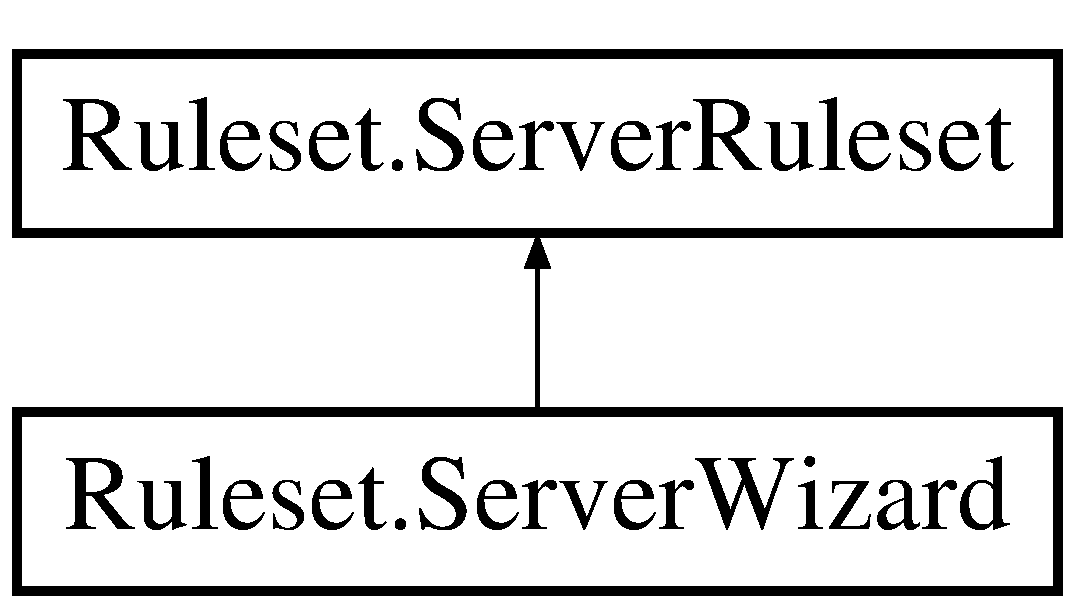
\includegraphics[height=2.000000cm]{a00017}
\end{center}
\end{figure}
\subsubsection*{Öffentliche Methoden}
\begin{DoxyCompactItemize}
\item 
boolean \hyperlink{a00017_af079641e9a83d29de9e1ac868a0af202}{is\-Valid\-Move} (\hyperlink{a00001}{Card} card)
\end{DoxyCompactItemize}


\subsubsection{Dokumentation der Elementfunktionen}
\hypertarget{a00017_af079641e9a83d29de9e1ac868a0af202}{\index{Ruleset\-::\-Server\-Wizard@{Ruleset\-::\-Server\-Wizard}!is\-Valid\-Move@{is\-Valid\-Move}}
\index{is\-Valid\-Move@{is\-Valid\-Move}!Ruleset::ServerWizard@{Ruleset\-::\-Server\-Wizard}}
\paragraph[{is\-Valid\-Move}]{\setlength{\rightskip}{0pt plus 5cm}boolean Ruleset.\-Server\-Wizard.\-is\-Valid\-Move (
\begin{DoxyParamCaption}
\item[{{\bf Card}}]{card}
\end{DoxyParamCaption}
)\hspace{0.3cm}{\ttfamily [virtual]}}}\label{a00017_af079641e9a83d29de9e1ac868a0af202}


Pr�ft ob ein gemachter Zug in einem Wizard Spiel g�ltig ist. 

\begin{DoxyReturn}{Rückgabe}
is\-Valid true falls Zug g�ltig, false wenn nicht 
\end{DoxyReturn}


Implementiert \hyperlink{a00016_aa49663b89f89b9f7b3685f0b96560f69}{Ruleset.\-Server\-Ruleset}.


\hypertarget{a00018}{\subsection{Other\-Player Klassenreferenz}
\label{a00018}\index{Other\-Player@{Other\-Player}}
}
\subsubsection*{Private Attribute}
\begin{DoxyCompactItemize}
\item 
\hypertarget{a00018_a46ff4804e1f3b2aa954327b7ebaedb5f}{Object {\bfseries name}}\label{a00018_a46ff4804e1f3b2aa954327b7ebaedb5f}

\item 
\hypertarget{a00018_a479739d676f2040870ad5be69a6c8a9e}{Object {\bfseries info}}\label{a00018_a479739d676f2040870ad5be69a6c8a9e}

\end{DoxyCompactItemize}


\subsubsection{Ausführliche Beschreibung}
Zeigt die Informationen über die anderen Spieler an, also den Namen, ein Symbol für die verdeckte Hand und das Label für zusaetzliche Angaben. 
\hypertarget{a00019}{\subsection{Own\-Hand Klassenreferenz}
\label{a00019}\index{Own\-Hand@{Own\-Hand}}
}
\subsubsection*{Private Attribute}
\begin{DoxyCompactItemize}
\item 
\hypertarget{a00019_a9233afadd1e46e11f03ea518e9c86366}{Object {\bfseries cards}}\label{a00019_a9233afadd1e46e11f03ea518e9c86366}

\item 
\hypertarget{a00019_a32963d9bbf9a4ad1ca8d0e1cf6c54bfe}{Set$<$ \hyperlink{a00022}{View\-Card} $>$ {\bfseries card}}\label{a00019_a32963d9bbf9a4ad1ca8d0e1cf6c54bfe}

\end{DoxyCompactItemize}


\subsubsection{Ausführliche Beschreibung}
Stellt die Karten dar, die der Spieler auf der Hand hat. Der Spieler kann eine Karte durch Anklicken auswaehlen und durch einen zweiten Klick ausspielen. 
\hypertarget{a00020}{\subsection{Com\-Objects.\-Com\-Client\-Leave Klassenreferenz}
\label{a00020}\index{Com\-Objects.\-Com\-Client\-Leave@{Com\-Objects.\-Com\-Client\-Leave}}
}
Klassendiagramm für Com\-Objects.\-Com\-Client\-Leave\-:\begin{figure}[H]
\begin{center}
\leavevmode
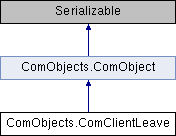
\includegraphics[height=3.000000cm]{a00020}
\end{center}
\end{figure}


\subsubsection{Ausführliche Beschreibung}
Sie wird zur Benachrichtigung gesendet, wenn ein Spieler ins nächste Fenster möchte und aus dem alten entfernt werden soll. 
%--- End generated contents ---

% Index
\newpage
\phantomsection
\addcontentsline{toc}{part}{Index}
\printindex

\end{document}
